%!TEX root = ../thesis.tex
%*******************************************************************************
%****************************** Third Chapter **********************************
%*******************************************************************************
\chapter{Electricity demand prediction}

% **************************** Define Graphics Path **************************
\ifpdf
    \graphicspath{{Chapter3/Figs/Raster/}{Chapter3/Figs/PDF/}{Chapter3/Figs/}}
\else
    \graphicspath{{Chapter3/Figs/Vector/}{Chapter3/Figs/}}
\fi

\section{Full paper}

\section{Introduction}

The energy markets have undergone significant changes in recent years. The liberalisation of the energy industry, technological advancements and policy changes have had a number of effects \cite{Viegas2016} including, a rise in both competition \cite{sioshansi_2009}, and quantity of data collected \cite{Clastres2011}, as well as a requirement to integrate large amounts of intermittent renewable resources \cite{Haben2013a,Kamgarpour2013,Curves2014}.

The need for accurate load forecasting is essential for control and planning of electricity generation in electrical grids due to the fact that supply must meet demand \cite{Lu1993}. Short-term electricity demand forecasting has become increasingly important due to the introduction of competitive energy markets. Accurate estimates of demand are required so that the correct amount of electricity is purchased on the wholesale market \cite{Dillon1991}. Electricity is unique to other commodities in that it must be either consumed the moment that it is generated or stored. The difficulties in storing electricity arise from high installation and maintenance costs, inefficiencies and low capacity \cite{Poonpun2008}. It is therefore important to match demand to supply and thus regulate frequency. Failure to accurately forecast electricity demand can lead to financial loss and/or system-wide blackouts \cite{Hines2008}.

The introduction of smart meters in many countries (USA, Europe, Canada and South Korea) has led to an influx of high granularity electricity consumption data that can be used for load forecasting \cite{Depuru2011a}. 800 million smart meters are projected to be installed worldwide by 2020 \cite{Telefonica2014}. Smart meters are digital devices that measure electricity consumption of individual households at regular intervals (intervals of an hour or less) and offer two-way communication between the meter and utility company. Smart meters aid customers to understand precisely how much electricity they consume at different time intervals, and enable dynamic pricing \cite{Abreu2012a}. Dynamic pricing allows utilities to charge varying prices at different times, for instance, charging a higher price when costly generation sources are used in times of peak demand, and lower prices at night time or weekends when demand is low \cite{Liu2016,Ito2013}. 

This paper explores short term load-forecasting at an interval of 30 minutes ahead and clusters similar users based on their electricity usage. A variety of different forecasting techniques were evaluated such as Random Forests \cite{TinKamHo}, Long-Short Term Memory neural networks (LSTM) \cite{lstm}, Multilayer Perceptron neural networks \cite{book:984557} and Support Vector Regression (SVR) \cite{Drucker1997}. 

Random Forests are an ensemble based learning method for classification and regression, and are made up of many decision trees. LSTM networks are recurrent neural networks which remember values over arbitrary time intervals. Multilayer Perceptrons are a popular type of neural network which are made up of a minimum of three layers and can be used to make non-linear predictions. SVR's are supervised learning models which analyze data used for regression analysis.

To improve forecasting results, the clustering of smart meter data was evaluated. The technique used for this was \textit{k}-means clustering. An average 24-hour electricity load profile was calculated, and the result used for clustering. The clustered sub-system is then aggregated and separate models trained on this aggregate. The yearly, weekly and daily periodicity of electricity load is accounted for by input variables into the models. Once forecasts for each cluster are made using the individual models, the results are aggregated for the final predictions. These predictions are compared to the actual results and the accuracy measured using mean absolute percentage error (MAPE).

This paper contributes a technique to forecasting smart-meter data through the use of clustering using \textit{k}-means and different learning algorithms. It provides researchers and utilities with methods to maximise forecasting accuracy through the selection of machine learning and clustering algorithms.

This paper is structured as follows: in Section 2 we introduce the state of the art in load forecasting. The methods used in this paper are explored in Section 3. The experiments and their evaluation are discussed in Section 4. The results are discussed in Section 5. In Section 6 we conclude and consider future directions for this work.

\section{Related Work}

The forecasting of aggregated and clustered electricity demand has been the focus of a considerable amount of research in recent years. The research can generally be classified into two classes, Artificial Intelligence (AI) techniques \cite{Kim2000, Tiong2008,Quilumba2014} and classical time series approaches \cite{Nazarko2005ARIMAApproach,Huang2003,Nguyen2017}. For the purposes of our paper we have evaluated artificial intelligence techniques.

Singh \textit{et al.} \cite{Singh2012} produced a review of load forecasting techniques and methodologies and reported that hybrid methods, which combine two or more different techniques, are gaining traction, as well as soft computing approaches (AI) such as genetic algorithms. Our paper presents a hybrid method which combines \textit{k}-means clustering with multiple different learning algorithms.

\subsection{Artificial Intelligence Techniques}

Dillon \textit{et al.} presented a neural network for short term load forecasting. Their neural network consisted of three-layers and used adaptive learning for training \cite{Dillon1991}. They proposed the use of weather information to augment their electricity load data. They found better results with the adaptive neural network than with a linear model, or non-adaptive neural network. In contrast to Dillon our paper focuses on a non-adaptive neural network and does not take into account weather information.

Chen \textit{et al.} used an Artificial Neural Network (ANN) to predict electricity demand of three substations in Taiwan. They integrated temperature data and reported that the best results when forecasting residential and commercial substations were during the week due to the influence of weather \cite{Chen1996}. In contrast to the work done by Chen \textit{et al.}, we focus on client-side prediction using smart meter data as opposed to substation data. We were, therefore, able to cluster the data based on load profile, as opposed to geographical location.


\subsection{Time Series Approach}

Al-Musaylh \textit{et al.} proposed the use of Support Vector Regression (SVR), an autoregressive integrated moving average (ARIMA) model and a multivariate adaptive regression spline (MARS) in their short term electricity demand forecasting system \cite{Al-Musaylh2018}. They found that for a half, and one-hour forecasting horizons, that the MARS model outperformed both the ARIMA and SVR.

Taylor evaluates different statistical methods including ARIMA, an adaptation of Holt-Winters' exponential smoothing \cite{Holt2004}, and an exponential smoothing method which focuses on the evolution of the intra-day cycle \cite{Taylor2008}. He found that the double seasonal adaptation of the Holt-Winters' exponential smoothing method was the most accurate method for short lead times between 10 and 30 minutes. 

In contrast to Taylor, Fard \textit{et al.} proposed a novel hybrid forecasting method based on both artificial intelligence and classical time series approaches. They utilised the wavelet transform, ARIMA and ANNs for short term load forecasting \cite{Fard2014}. The ARIMA model is created by finding the appropriate order using the Akaike information criterion \cite{Akaike1974}. The ARIMA model models the linear component of the load time series, and the residuals contain the non-linear components. These residuals are then decomposed by the discrete wavelet transform into its sub-frequencies. ANNs are then applied to these sub-frequencies and the outputs of both the ANN and ARIMA models are summed to make the final prediction. They found that this hybrid technique outperformed traditional methods. Our paper, however, does not integrate artificial intelligence and classical time series techniques.

\subsection{Clustering}

Multiple techniques have been proposed for the clustering of electricity load data prior to forecasting. Both Shu and Luonan, and Nagi \textit{et al.} propose a hybrid approach in which self-organizing maps are used to cluster the data, and Support Vector Regression is used to make predictions \cite{Shu2006,Tiong2008}. This technique proved robust for different data types, and was able to tackle the non-stationarity of the data. Shu showed that this hybrid approach out-performed a single SVR technique, whilst Nagi showed superior results to a traditional ANN system. In contrast to both Nagi \textit{et al.} and Shu and Luonan our paper utilises \textit{k}-means as the clustering algorithm 

Similarly to us, Quilumba \textit{et al.} proposed a \textit{k}-means clustering algorithm to cluster similar load profiles \cite{Quilumba2014}. They found that clustering does improve accuracy, and found an optimum number of 3 clusters.

Wijaya \textit{et al.} demonstrated that implementing clusters improved load-forecasting accuracy up to a certain level \cite{Wijaya2010}. Whilst, a study by Ili\'c \textit{et al.} showed that increasing the number of clusters did not improve accuracy \cite{Ilic2013}.


\section{Time series forecasting methods}

In this section, the basic principles behind ANNs, Support Vector Regression and Random Forests are discussed.

\subsection{Artificial Neural Network}


\begin{figure}
	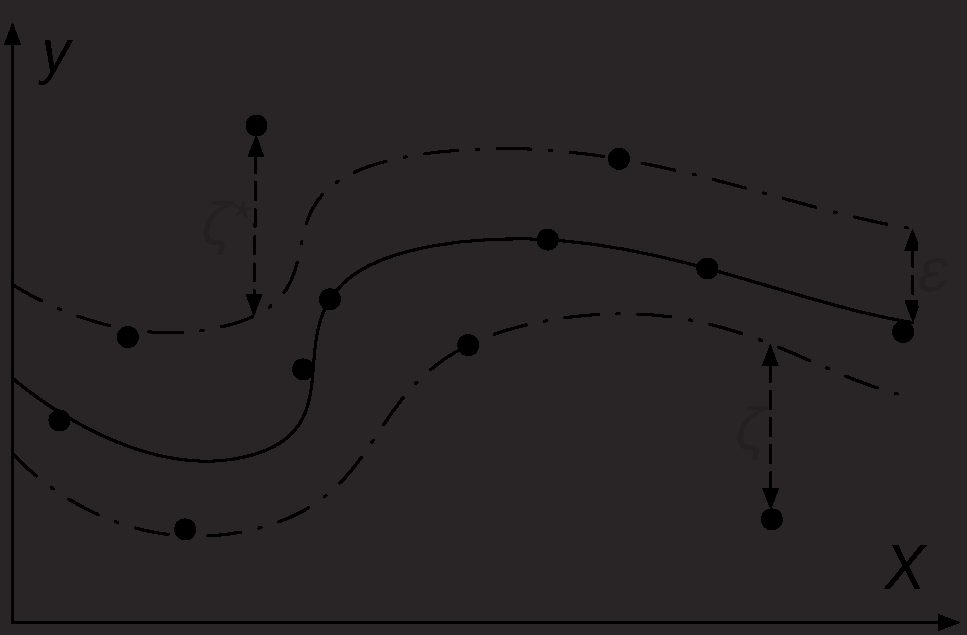
\includegraphics[width=0.8\textwidth]{Chapter5/figures/Kell_eEnergy_Fig2.pdf}
	\caption{A three layer feed forward neural network.}
	\label{fig:mlp}
\end{figure}


Artificial Neural Networks are a type of model which allow for non-linear relationships to be modeled between the input and output data \cite{Akaike1974}. A popular neural network is a feed forward multilayer network. Fig. \ref{fig:mlp} shows a three layer feed forward neural network with a single output unit, \textit{k} hidden units, $n$ input units. $w_{ij}$ is the connection weight from the $i$th input unit to the $j$th hidden unit,  and $T_j$ is the connecting weight from the $j$th hidden unit to the output unit \cite{Pao2007}. These weights transform the input variables in the first layer to the output variable in the final layer based upon the training data. 

Typically, a dataset is split into three sections, the test set, training set and validation set. The training set is used to find the connection weights of the network, whilst the test set is used to determine the accuracy of the models. The validation set allows for an unbiased evaluation of the model whilst tuning the hyperparameters, and can avoid overfitting by stopping training if the error begins to increase.

For a univariate time series forecasting problem, suppose we have N observations $y_1, y_2, \ldots, y_N$ in the training set, 
\begin{equation}
y_{N+1}, y_{N+2}, \ldots, y_{N+m}
\end{equation}
\noindent in the test set and we are required to predict \textit{m} periods ahead \cite{Pao2007}. 

The training patterns are as follows:
\begin{align}
y_{p+m} & =f(y_p, y_{p-1},\ldots,y_1)\\
y_{p+m+1} & =f(y_{p+1}, y_{p},\ldots,y_2)\\
&\vdotswithin  \notag \\
y_{N} & =f(y_{N-m},y_{N-m-1},\ldots,y_{N-m-p+1})
\end{align}

\noindent where $f$ is the function made up of weights and activation functions in the trained neural network.

The $m$ testing patterns are 

\begin{align}
y_{N+1} & =f(y_{N+1-m}, y_{N-m},\ldots,y_{N-m-p+2})\\
y_{N+2} & =f(y_{N+2-m}, y_{N-m+1},\ldots,y_{N-m-p+3})\\
&\vdotswithin  \notag \\
y_{N+m} & =f(y_{N},y_{N-1},\ldots,y_{N-p+1})
\end{align}

The training objective is to minimize the overall predictive error means (SSE) by adjusting the connection weights. For this network structure the SSE can be written as:
\begin{equation}
SSE = \sum_{i=p+m}^N(y_i-\hat{y}_i)
\end{equation}

\noindent where $\hat{y}_i$ is the output from the network. The number of input nodes corresponds to the number of lagged observations. Having too few or too many input nodes can affect the predictive ability of the neural network \cite{Pao2007}.




\subsection{Support Vector Regression}

A Support Vector Regression model maps input data, $x$, into a higher-dimensional feature space non-linearly. Given the input data:

\begin{equation}
(x_1,y_1), \ldots,(x_i,y_i),\ldots,(x_n,y_n) 
\end{equation}

\noindent where $x_i$ is the input, and $y_i$ is the output value of $x_i$. Support Vector Regression solves an optimization problem \cite{Shu2006,Chen2004}

\begin{equation}
\min_{\omega,b,\xi,\xi^{*}}\frac{1}{2}\omega^T\omega+C\sum_{i=1}^{n}(\xi_i+\xi_i^*)
\end{equation}

\noindent subject to
\begin{align}
\begin{multlined}
\label{svr:constrains}
y_i-(\omega^T\phi(x_i)+b)\leq\varepsilon+\xi_i^{*},\\
(\omega^T\phi(x_i)+b)-y_i\leq\varepsilon+\xi_i,\\
\xi_i,\xi^*_i\geq0,i=1,\ldots,n
\end{multlined}
\end{align}


\noindent $x_i$ is mapped to a higher dimensional space using the function $\phi$. The $\varepsilon$-insensitive tube $(\omega^T\phi(x_i)+b)-y_i\leq\varepsilon$ is a range shown in Figure \ref{fig:insensitive} in which errors are permitted. $\xi_i$ and $\xi^*_i$ are slack variables which allow errors for data points which fall outside of $\varepsilon$. This enables the optimisation to take into account the fact that data does not always fall within the $\varepsilon$ range \cite{Smola2004}.

The constant $C>0$ determines the trade-off between the flatness of the support vector function. $\omega$ is the model fit by the SVR. The parameters which control regression quality are the cost of error $C$, the width of the tube $\varepsilon$, and the mapping function $\phi$ \cite{Shu2006,Chen2004}. 

Figure \ref{fig:insensitive} demonstrates this principle, where only data points which fall outside of the $\varepsilon$-insensitive tube are penalised in the cost function

\begin{figure}[b]
	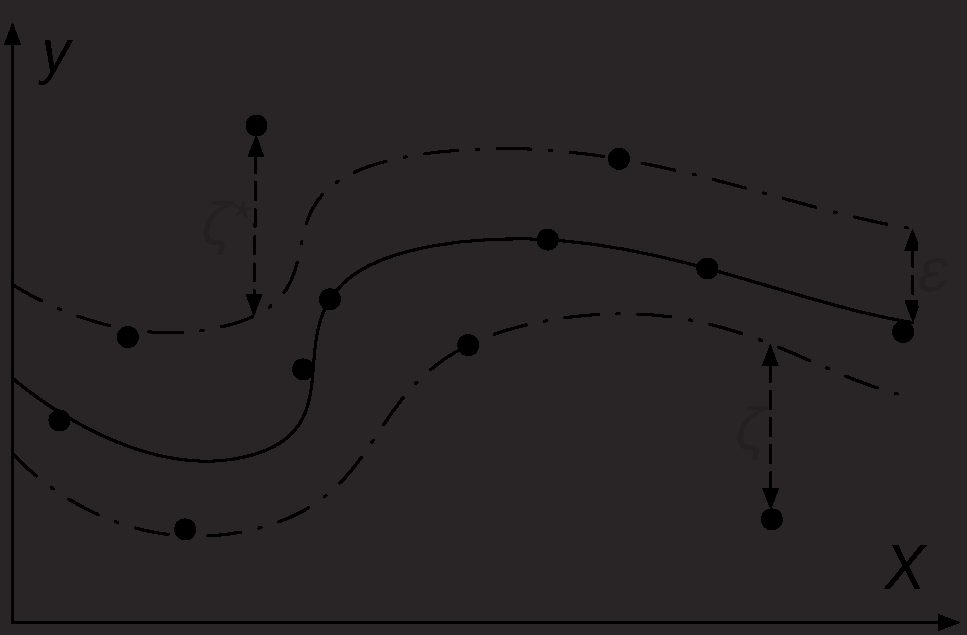
\includegraphics[width=0.8\textwidth]{Chapter5/figures/Kell_eEnergy_Fig2.pdf}
	\caption{$\varepsilon$-insensitive band for SVR \cite{Shu2006}.}
	\label{fig:insensitive}
\end{figure}

The constraints shown in \eqref{svr:constrains} imply that most of the data $x_i$ falls within the tube $\varepsilon$. By minimizing the training error $C\sum_{i=1}^n(\xi_i+\xi_i^*)$, and the regularisation term $\frac{1}{2}\omega^T\omega$, under-fitting and over-fitting are avoided. 

Due to the fact that $\phi$ maps $x_i$ to a high or infinite dimensional space, $\omega$ can be solved, subject to the constraints in \eqref{svr:constrains}, by Lagrangian optimisation. Thus the dual problem is solved \cite{Shu2006,Chen2004,Smola2004}:

\begin{align}
\min_{\alpha\alpha^*}\frac{1}{2}(\alpha-\alpha^*)^TQ(\alpha-\alpha^*)+\varepsilon\sum^n_{i=1}(\alpha_i+\alpha_i^*)+\sum_{i=1}^ny_i(\alpha_i-\alpha_i^*)
\end{align}

\noindent subject to 
\begin{align}
\begin{multlined}
\sum_{i=1}^n(\alpha_i-\alpha_i^*)=0,\\
0\leq\alpha_i,\alpha^*_i\leq C,i=1,\ldots,n
\end{multlined}
\end{align}

\noindent where $Q_{ij}=\phi(x_i)^T\phi(x_j)$, $a_i$ and $a_i^*$ are Lagrange multipliers. However due to the large number of elements in $\phi(x)$ we apply a "kernel trick" to do the mapping implicitly. Now, the optimisation can be calculated using solely dot products. An example of the linear function kernel is listed below, which is used in this paper:
\begin{equation}
K(x,y)=x^Ty.
\end{equation}

\subsection{Decision Tree}

A decision tree is a statistical model used for either classification or regression \cite{breiman1984classification}. Load forecasting is a regression problem, and therefore regression trees are used in this paper. 

Decision trees recursively partition data into nodes with different labels until the termination criteria is met. This is typically initiated when it is not possible to have children nodes with different output labels. The terminal nodes are known as leaves and they represent the different outputs.

\subsection{Random Forest}

A Random Forest is an ensemble method that combines the predictions of many decision trees \cite{Breiman2001}. Each decision tree is fit by a random sample, with replacement, of the training data. The final decision of the Random Forest is decided by a majority case wins vote on each of the decision trees.


\subsection{MAPE}

For the measure of prediction accuracy, this paper adopts mean absolute percentage error (MAPE). The formula is as follows:

\begin{equation}
MAPE=\frac{1}{n}\sum_{i=1}^n\left|\frac{y_i-\hat{y}_i}{y_i}\right|\times 100\%
\end{equation}

\noindent where $y_i$ is the actual value, $\hat{y}_i$ is the forecast value and $n$ is the number of points forecast \cite{Li2016}.

\subsection{Root Mean Squared Error}

The root mean squared error (RMSE) is a measure between the values predicted by a model and the observed values. The RMSE is the sample standard deviation of the differences between the predicted and observed values.

The RMSE is defined as follows:
\begin{equation}
RMSE = \sqrt[]{\frac{\sum_{t=1}^n(\hat{y}_i-y_i)^2)}{n}}
\end{equation}

\noindent where $\hat{y}_i$ are the predicted values, $y_i$ are the observed values, and $n$ is the number of observations.


\section{Methodology}

In this section, we will present the methodology for the approach taken in this paper. 

The work in this paper was run on a MacBook Pro with a quad-core 3.1GHz Intel Core i7 processor with 16 GB 1867 MHz DDR3 of RAM and a 500GB solid state drive (SSD).

\subsection{Data Collection}


Smart meter data obtained from the Irish Social Science Data Archive (ISSDA) on the 28th of September 2017 was used in this study \cite{cer_2012}. The Commission for Energy Regulation released a public dataset of anonymised smart meter data from the "\textit{Electricity Smart Metering Customer Behaviour Trials}" \cite{setis}. This dataset is made up of over 5000 Irish homes and businesses and is sampled at 30-minute intervals.

The data was recorded between the 14th July 2009 and 31st December 2010, providing 17 months worth of data. For the purposes of cross-validation the data was split into two partitions, the training set and the testing set. The training set made up the first 11 months of data and was used to parametrise the models, whereas the test set is made up of the remaining 6 months of data. This split was chosen to balance the amount of training data with the test data and to give the models a chance to learn the periodicity inherent in a one year period of electricity load. The test set was used for evaluation of the models proposed. Due to the long training times for these algorithms, we worked with a sub-sample of 709 individual Irish homes from the whole dataset. However, we believe that our results would hold over the full dataset.

\begin{figure}[b]
	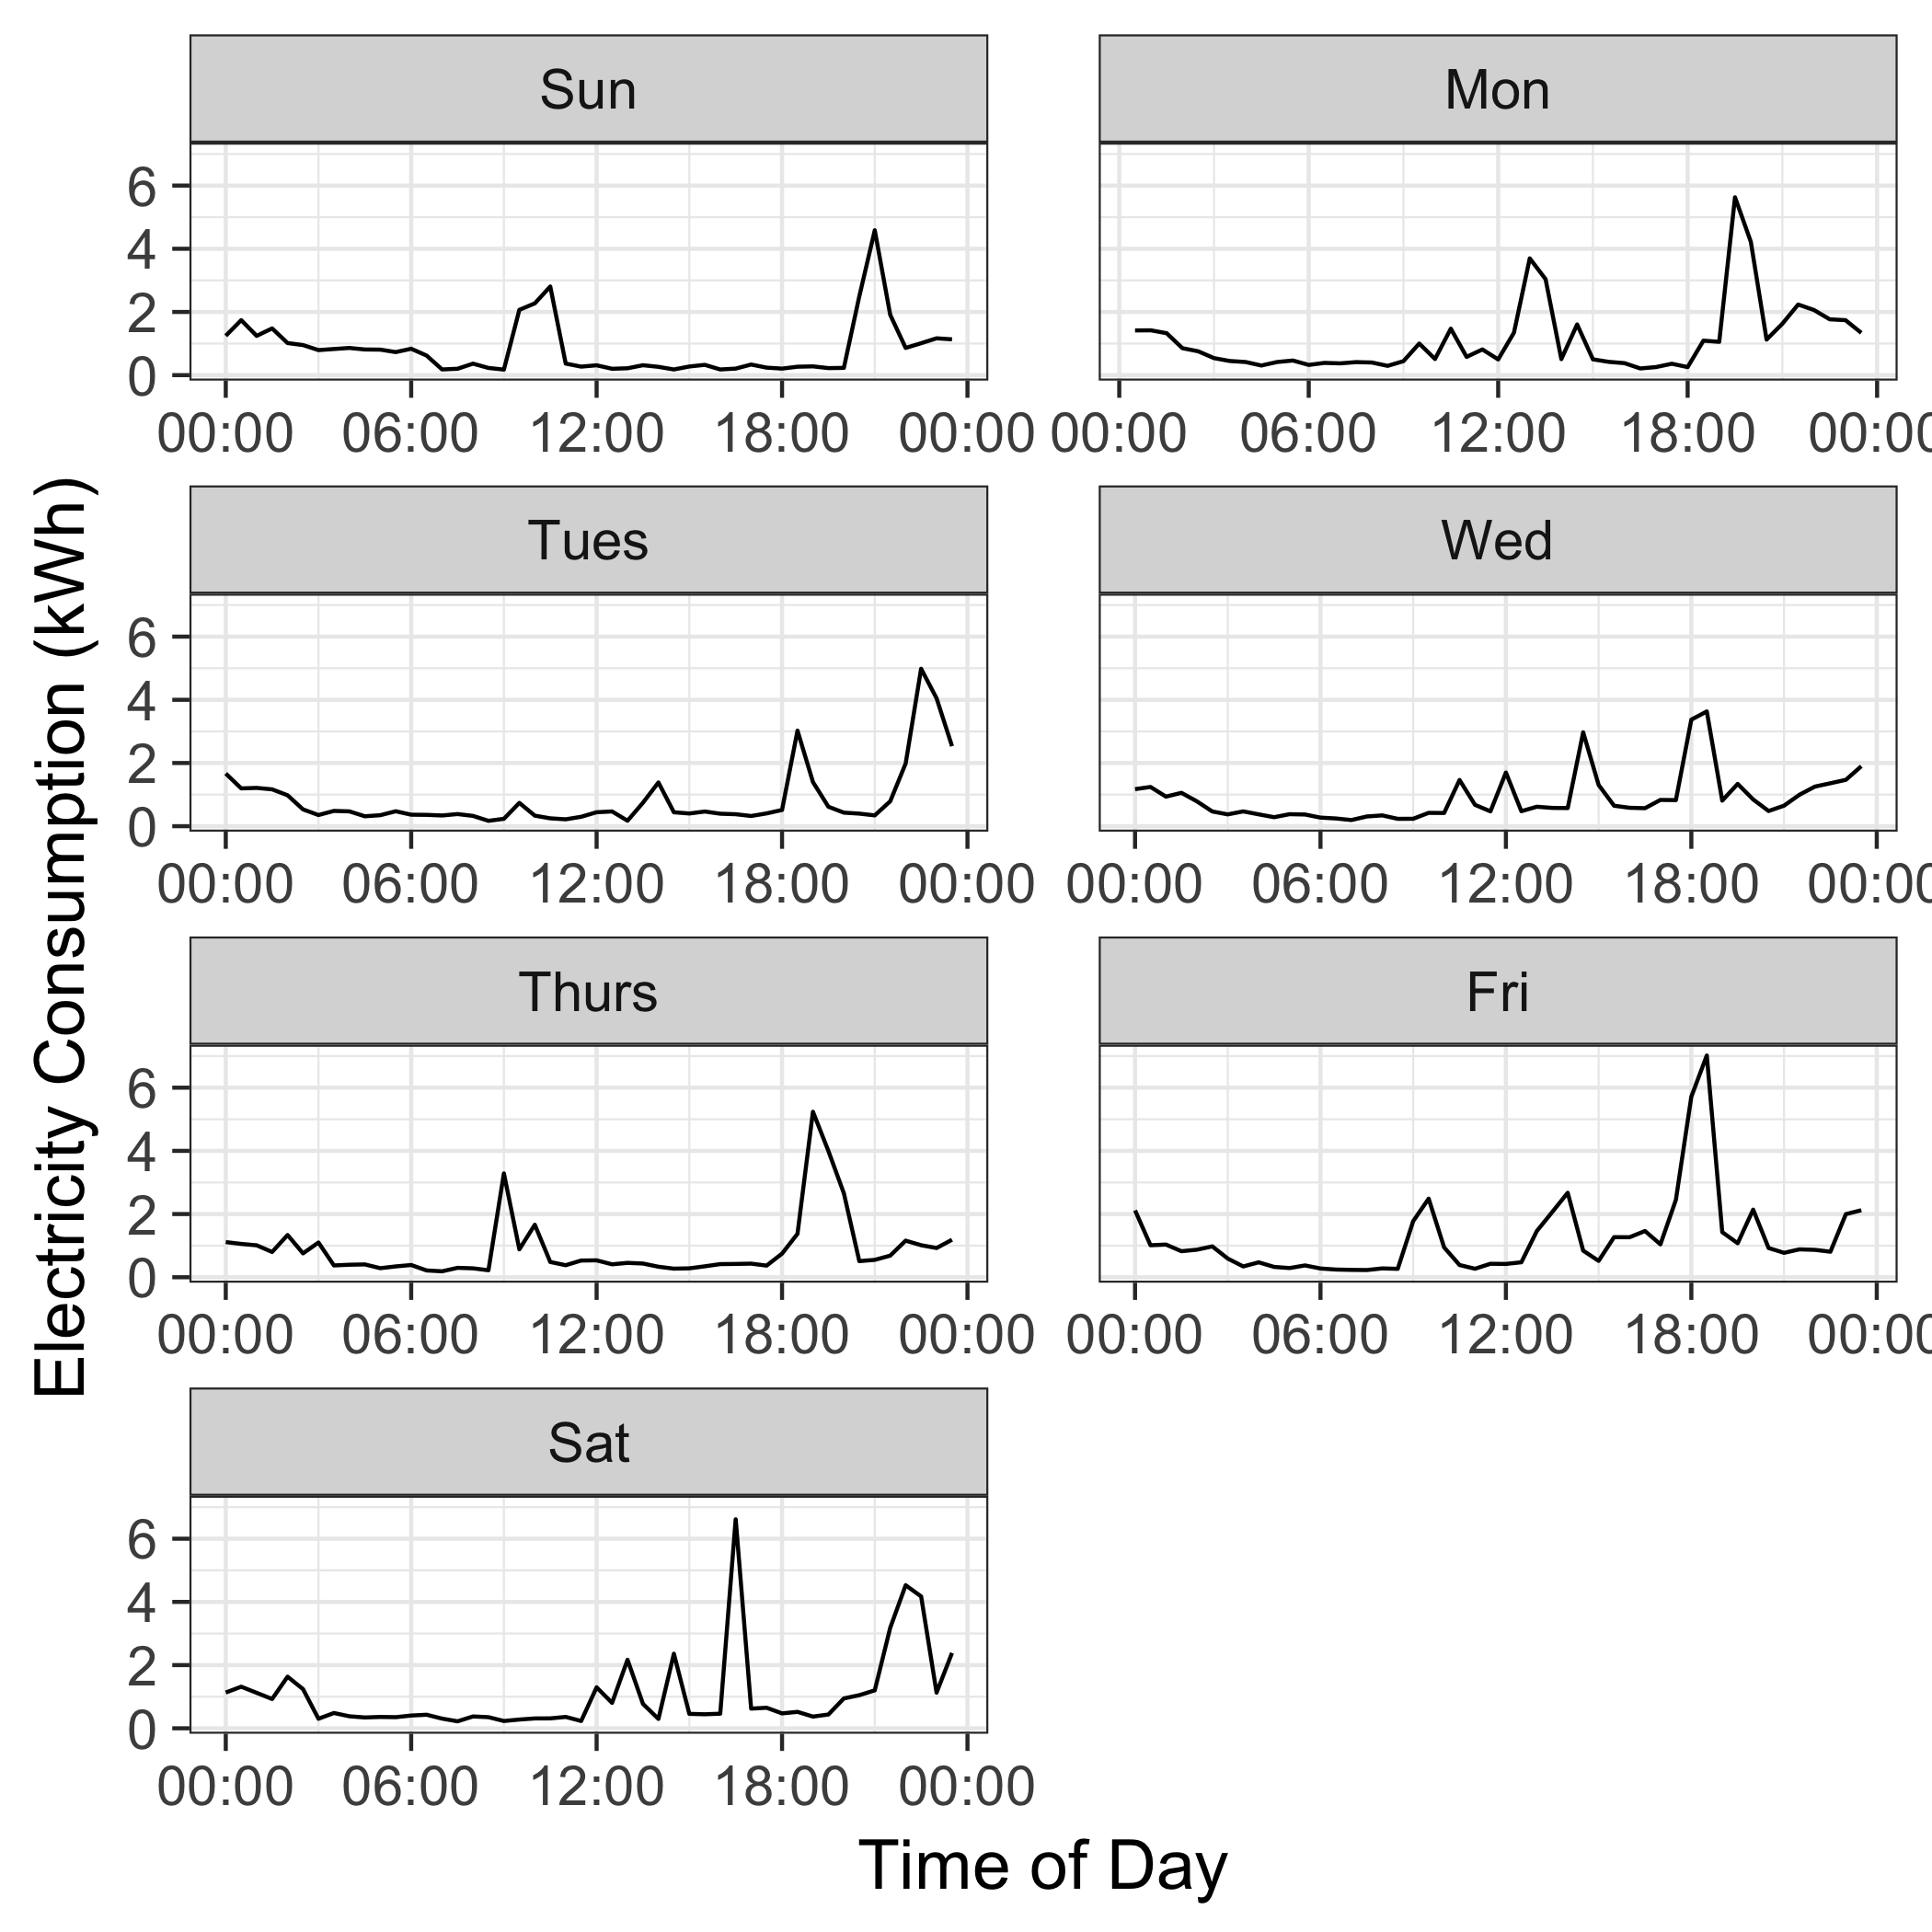
\includegraphics[width=0.8\textwidth]{Chapter5/figures/Rplot01.png}
	\caption{Daily load profiles of a single customer over a week between 20th July 2009 and 27th July 2009. }
	\label{fig:single_user}
\end{figure}

Figure \ref{fig:single_user} demonstrates the electricity consumption profile of a single week for a single user. Whilst it can be seen that electricity usage changes significantly between days, a pattern of behaviour is exhibited. There is a large peak displayed each day in the evening, as well as a peak earlier during the day. It can, therefore, be assumed that this customer has some form of habitual behavioural pattern. 

Figure \ref{fig:multiple_users} shows eight different residential customer load profiles on the 22nd June 2009. It can be seen that the daily load profile changes between each customer. The consumers use varying quantities of electricity and at different times. 




\begin{figure}
	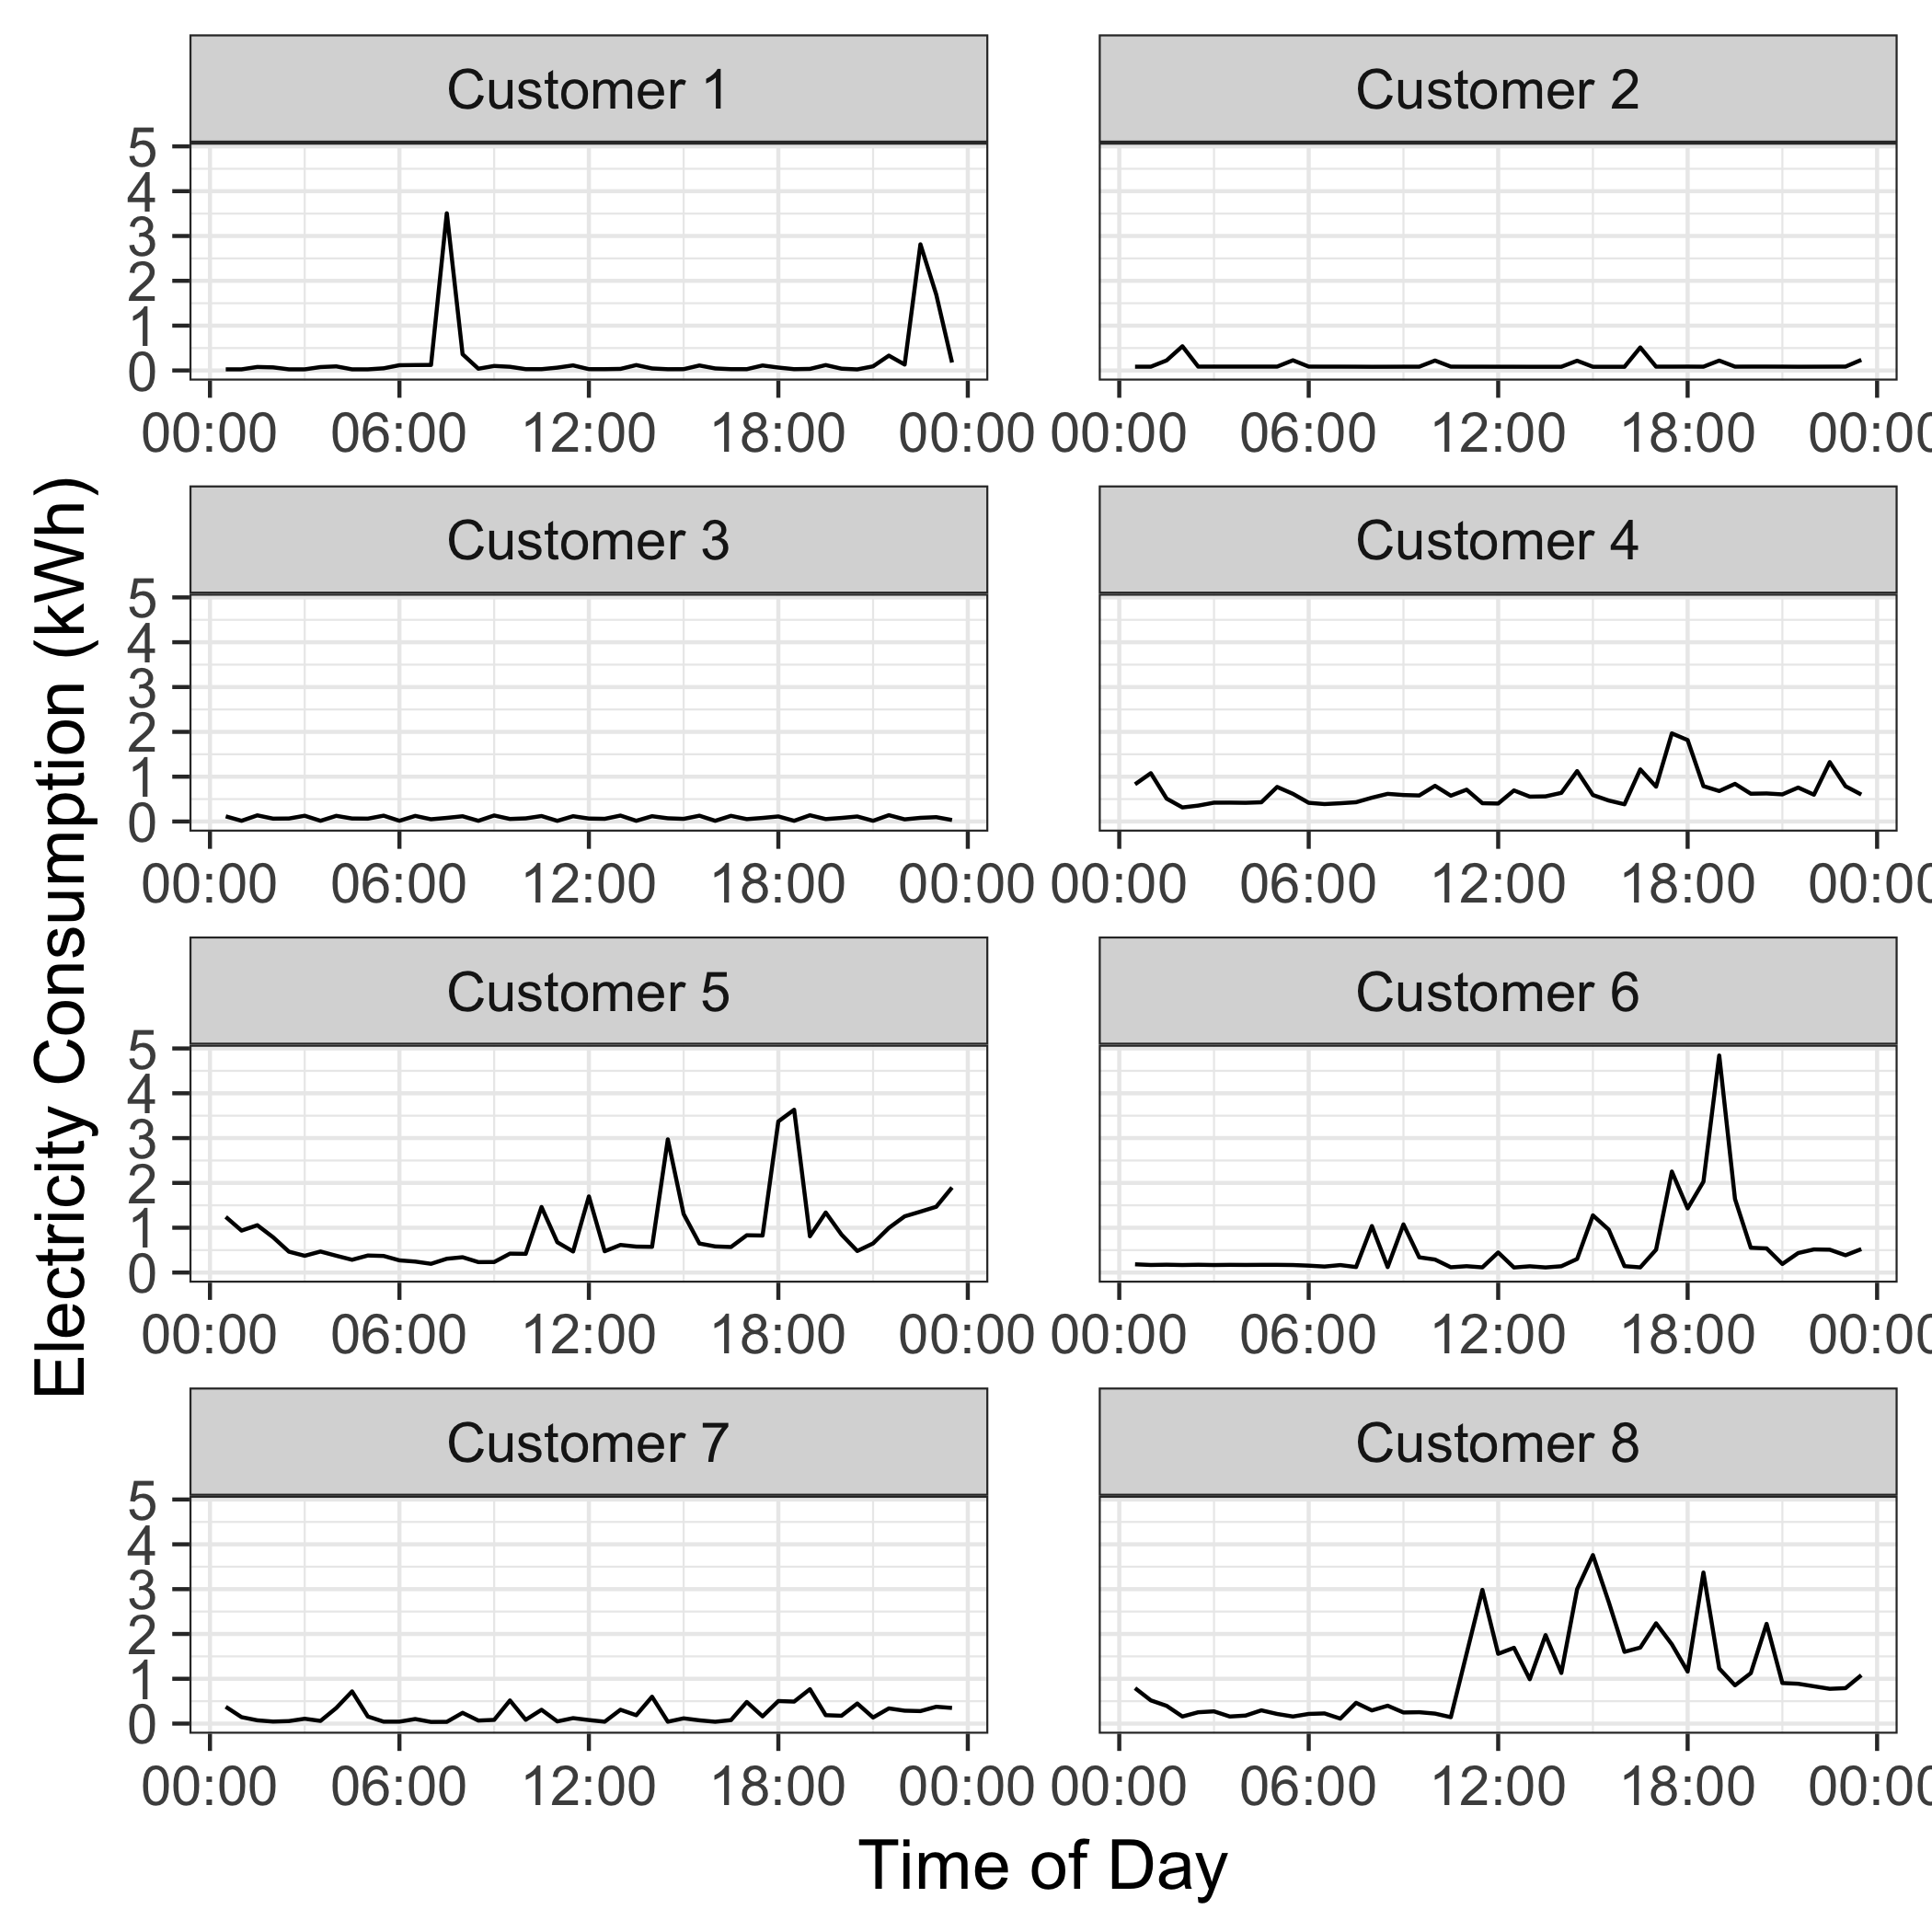
\includegraphics[width=0.8\textwidth]{Chapter5/figures/Rplot02.png}
	\caption{Daily load profiles of different customers over a single day on the 22nd June 2009.}
	\label{fig:multiple_users}
\end{figure}

These figures display that electricity consumption changes per person, per day. To capture this variability between customer types these customers are clustered and then aggregated. Each of the different aggregated electricity consumptions should provide a less stochastic load profile, and therefore increase the accuracy of the models.

\subsection{Clustering}

We propose that clustering similar customer load profiles and aggregating each cluster's electricity consumption improves the accuracy of the models. 

Figure \ref{fig:similar_customers} displays four different customers with similar load profiles. Each of the users display a strong peak in electricity consumption during the evening and less consumption during the day. These customers may potentially be clustered together by the \textit{k}-means clustering algorithm.

\begin{figure}[b]
	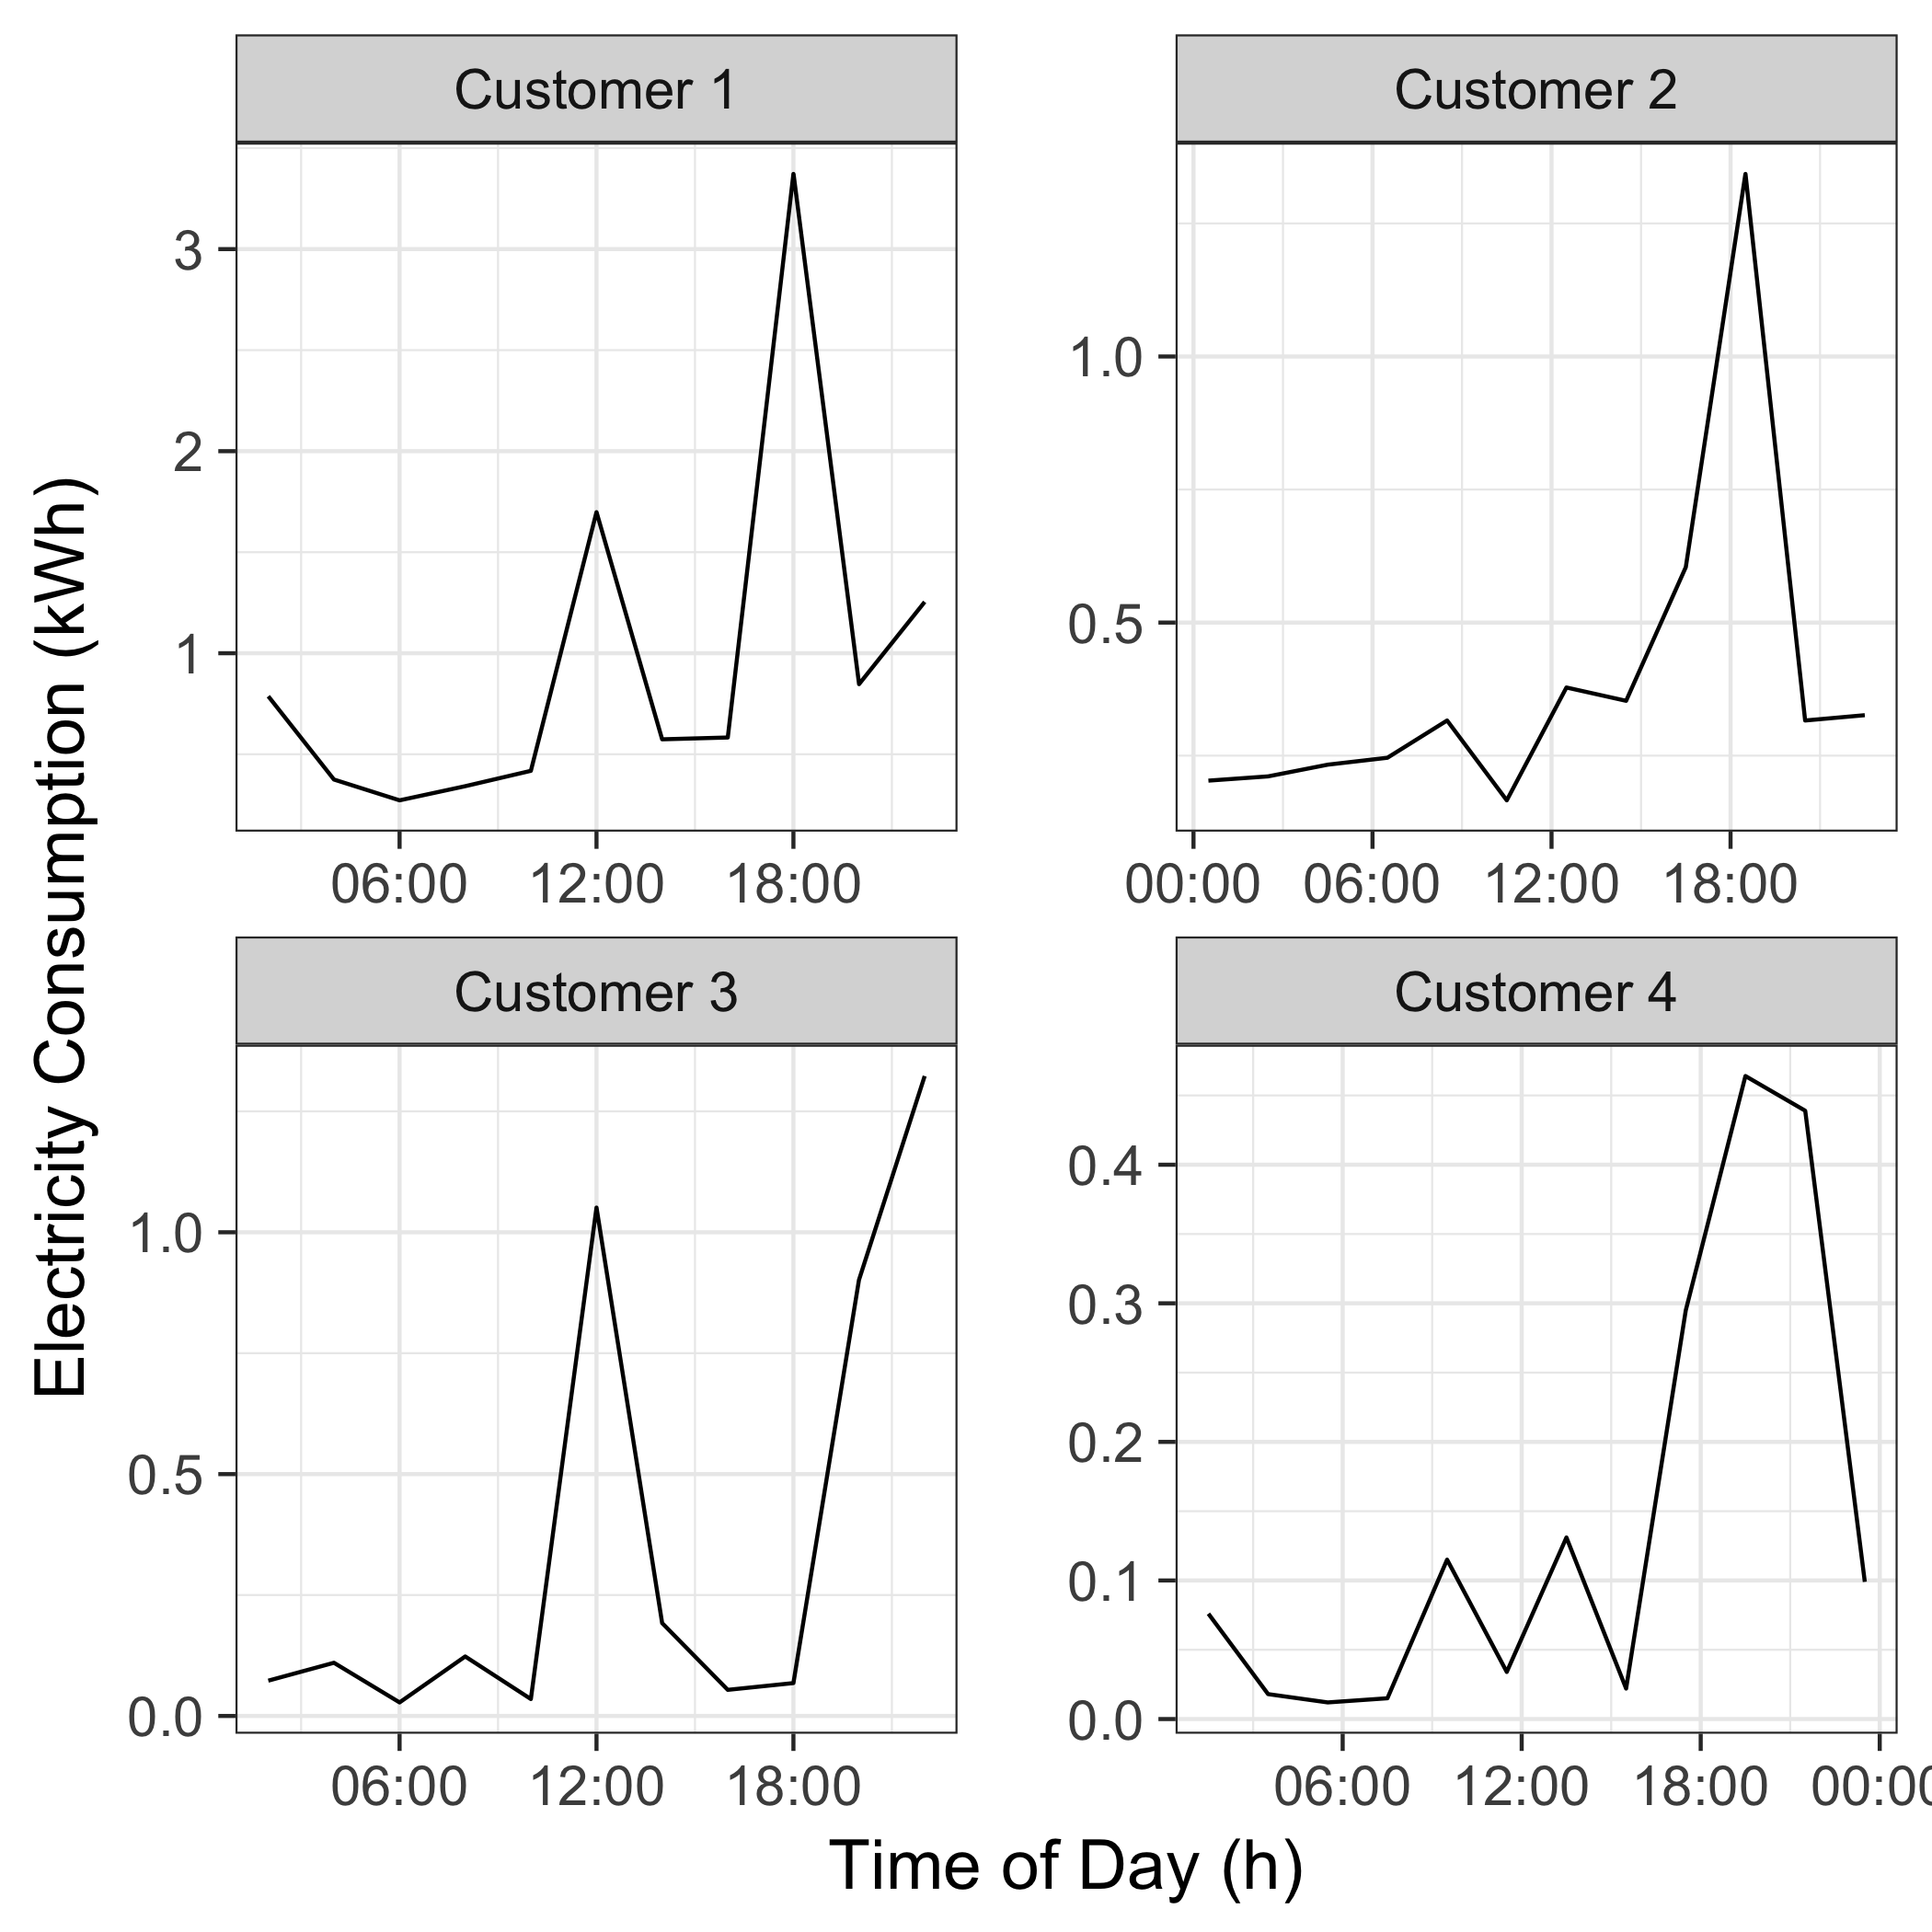
\includegraphics[width=0.45\textwidth]{Chapter5/figures/similar_cust.png}
	\caption{Figure showing similar load profiles for four different customers on the 22nd July 2009.}
	\label{fig:similar_customers}
\end{figure}

To cluster the load profiles different options were considered. Hierarchical clustering using metrics such as Euclidean and wavelet distance metrics were evaluated \cite{BIMJ:BIMJ4710240520}, as was \textit{k}-means \cite{Forgy65}.\textit{ K}-means demonstrated to be the most robust and best-performing clustering algorithm, and thus was chosen for use in this paper.

To select the optimum number of clusters (\textit{k}) cross-validation was explored. This allowed us to compare the results of each of the models and select \textit{k} with the highest MAPE accuracy.

The cross-validation method proposed, worked by trying a different number of clusters per model, and testing for the resulting MAPE. The optimum number of clusters with a low MAPE is then chosen. In this paper we varied \textit{k} between 1 and 7, this range was chosen due to the fact that the error did not vary greatly past seven clusters. We fit multiple models per cluster and predicted 6 months of electricity consumption.

With \textit{k}-means clustering, it is possible that with the same initialization number of clusters, different clusters are formed. This is due to the algorithm converging at a local minima. To overcome local minima the \textit{k}-means algorithm is run multiple times and the partition with the smallest squared error is chosen \cite{Jain2010}. In our case, the \textit{k}-means clustering algorithm is run 1000 times to reduce the chance of finding a local minima. 

The clustering technique utilised in our paper was a scaled input approach. The daily load profile was averaged for each customer based on each day of the training data. The data was then scaled so that households of different sizes, but with similar usage profiles were clustered together. This data, which is made up of a \textit{m-by-n} matrix, where \textit{m} is equal to the total number of meters and \textit{n} is equal to 48 (two readings for each hour in the day).

To find the optimum number of clusters it is recommended that the user selects a value of $k$ that is high enough that distinct average load profiles are displayed, however, not so high that well-clustered customers are split. By doing this, the stochasticity of the load profiles in each of the clusters will be reduced, and thus lead to the best results.


\subsection{Aggregating Demand}

Once each customer is assigned to their respective cluster, the total electricity consumed per cluster is aggregated. This is achieved by summing the electricity consumed at each time interval per cluster. This creates a partial system load. A different model is trained on each of the different partial system loads, and the resultant forecasts are aggregated to generate the total system load forecast. The total system load forecast is then used to evaluate the accuracy of each of the different models using MAPE. 

Random Forests, Support Vector Regression, Multilayer Perceptron neural networks and Long-Short Term Memory neural networks were evaluated, and a comparison between the different models were made. 

These models were chosen due to their ability to model multivariate non-linear relationships. They are data-driven methods and therefore suited to this type of problem.

\subsection{Feature Selection}

Each component of the training data is known as a feature. Features encode information from the data that may be useful in predicting electricity consumption. 

\subsubsection{Calendar Attributes}

Due to the daily, weekly and annual periodicity of the electricity consumption daily calendar attributes may be useful to model the problem. The calendar attributes included are as follows:

\begin{itemize}
	\item Hour of day
	\item Day of the month
	\item Day of the week
	\item Month
	\item Public holidays
\end{itemize}

These attributes enable the daily, weekly and annual periodicity to be taken into account by the model.

It is noted that electricity consumption changes on a public holiday such as Christmas or New Year's Eve. It is therefore proposed that public holidays in Ireland are input into the model as features. 

For testing purposes, two sets of models for Random Forests, Multilayer Perceptrons and Support Vector Regression were fit. One set omitted these calendar attributes whilst the other didn't. This is done to evaluate the importance of periodicity in electricity consumption prediction.

\subsubsection{Time Series Data}

As well as the calendar attributes it is important to consider the historical load demand. This allows the time-series element to be modelled.  

To do this, a lagged input of the previous 3 hours, the equivalent three hours from the previous day, and the equivalent 3 hours from the previous week were used. For example, to predict the electricity consumed on the 21st December 2010 at 12:00 pm the electricity between 9:00 pm and 11:30 pm on the 21st of December are used as inputs, as are the times between 9:00 pm and 12:00 pm on the 20th and 14th of December.

Long-Short Term Memory neural networks remember values over arbitrary time intervals. They can remember short-term memory over a long period of time, for this reason, 5 lagged inputs of the previous two and a half hours were used as features to the Long-Short Term Memory network.

\subsubsection{Data Representation}

Once useful information is selected we must encode the data for input into the models. To encode the day of the week seven binaries are utilised. Six of the binaries are for Monday through to Saturday. When all six binaries are equal to zero Sunday is encoded. A single binary for public holidays is included. Eleven binaries are used for month of the year, with the first eleven representing January to November, with December represented by all zeros in the calendar binaries. The current hour and date are input using a numerical attribute. The lagged data inputs, such as previous hour's electricity usage are also input using a numerical attribute for each entry, totaling 20 attributes (six half hourly entries for each 3 hour period multiplied by three days plus 2 entries for the time to be predicted on the previous day and week). Table \ref{tab:feature} displays these features.


\begin{table}
	\caption{List of Input Data for Models}
	\label{tab:feature}
	\begin{tabular}{p{3cm}p{5cm}p{8cm}}
		\toprule
		Input & Variable      & Detail description \\
		\midrule
		1     & Hour          & Single numeric input representing hour of the day                                                                                              \\
		2     & Day of month  & Single numeric input representing day of the month                                                                                             \\
		3-9   & Day of week   & Six binary digits representing calendar information regarding day of the week                                                                                            \\
		10-21 & Month         & Eleven binary digits representing calendar information regarding month                                                                                         \\
		22-42 & Lagged inputs & Twenty numeric inputs representing lagged inputs of previous 3 hours, previous 3 hours of previous day including hour to be predicted, and previous 3 hours of previous week including hour to be predicted \\
		43    & Holiday       & One binary digit representing whether the day was a public holiday  \\     \bottomrule                                                           
	\end{tabular}
\end{table}


\subsection{Experiments}

This section explores the different methods used to select the model parameters, and the tests to evaluate our models. Once the parameters were chosen the models were trained on the different clusters of residential customers. Each model was run five times to explore the variance of the results.  

\subsubsection{Support Vector Regression}

To implement a Support Vector Regression model a variety of parameters must be chosen. These parameters influence the performance of the model. The parameters were evaluated using cross-validation. To do this, the data was split 75\% into training data, and the remaining 25\% into test data. This split was chosen to balance the trade-off between having enough training data so that the model can accurately learn the underlying form of the data, but also to have enough data to test each model.

To choose the optimum support vector machine kernel cross-validation was also used. Again, with 75\% acting as the training data and 25\% as the test. The kernels compared were polynomial, radial basis function (RBF) and the linear kernel \cite{Chang2010, theodoridis2009pattern}. These were chosen due to their popularity, support and relative speed of computation.

The parameter values selected are shown in Table \ref{tab:kernel}. These parameter values were chosen from the results of cross-validation for each of the different kernels.  From the cross-validation, the linear kernel was found to be the best performing. For this reason, the linear kernel was utilised for prediction of electricity consumption in this paper.

\begin{table}
	\caption{Prediction Accuracy Based on Type of Kernel}
	\label{tab:kernel}
	\begin{tabular}{ccl}
		\toprule
		Kernel Type& Kernel Parameters & RMSE\\
		\midrule
		Linear & No values & 0.02103\\
		RBF & C=2, $\gamma=0.016$ & 0.0245\\
		Polynomial & C=2, $d=2, r=2$ & 0.0315 \\
		\bottomrule
	\end{tabular}
\end{table}


\subsubsection{Random Forest}

\begin{figure}[b]
	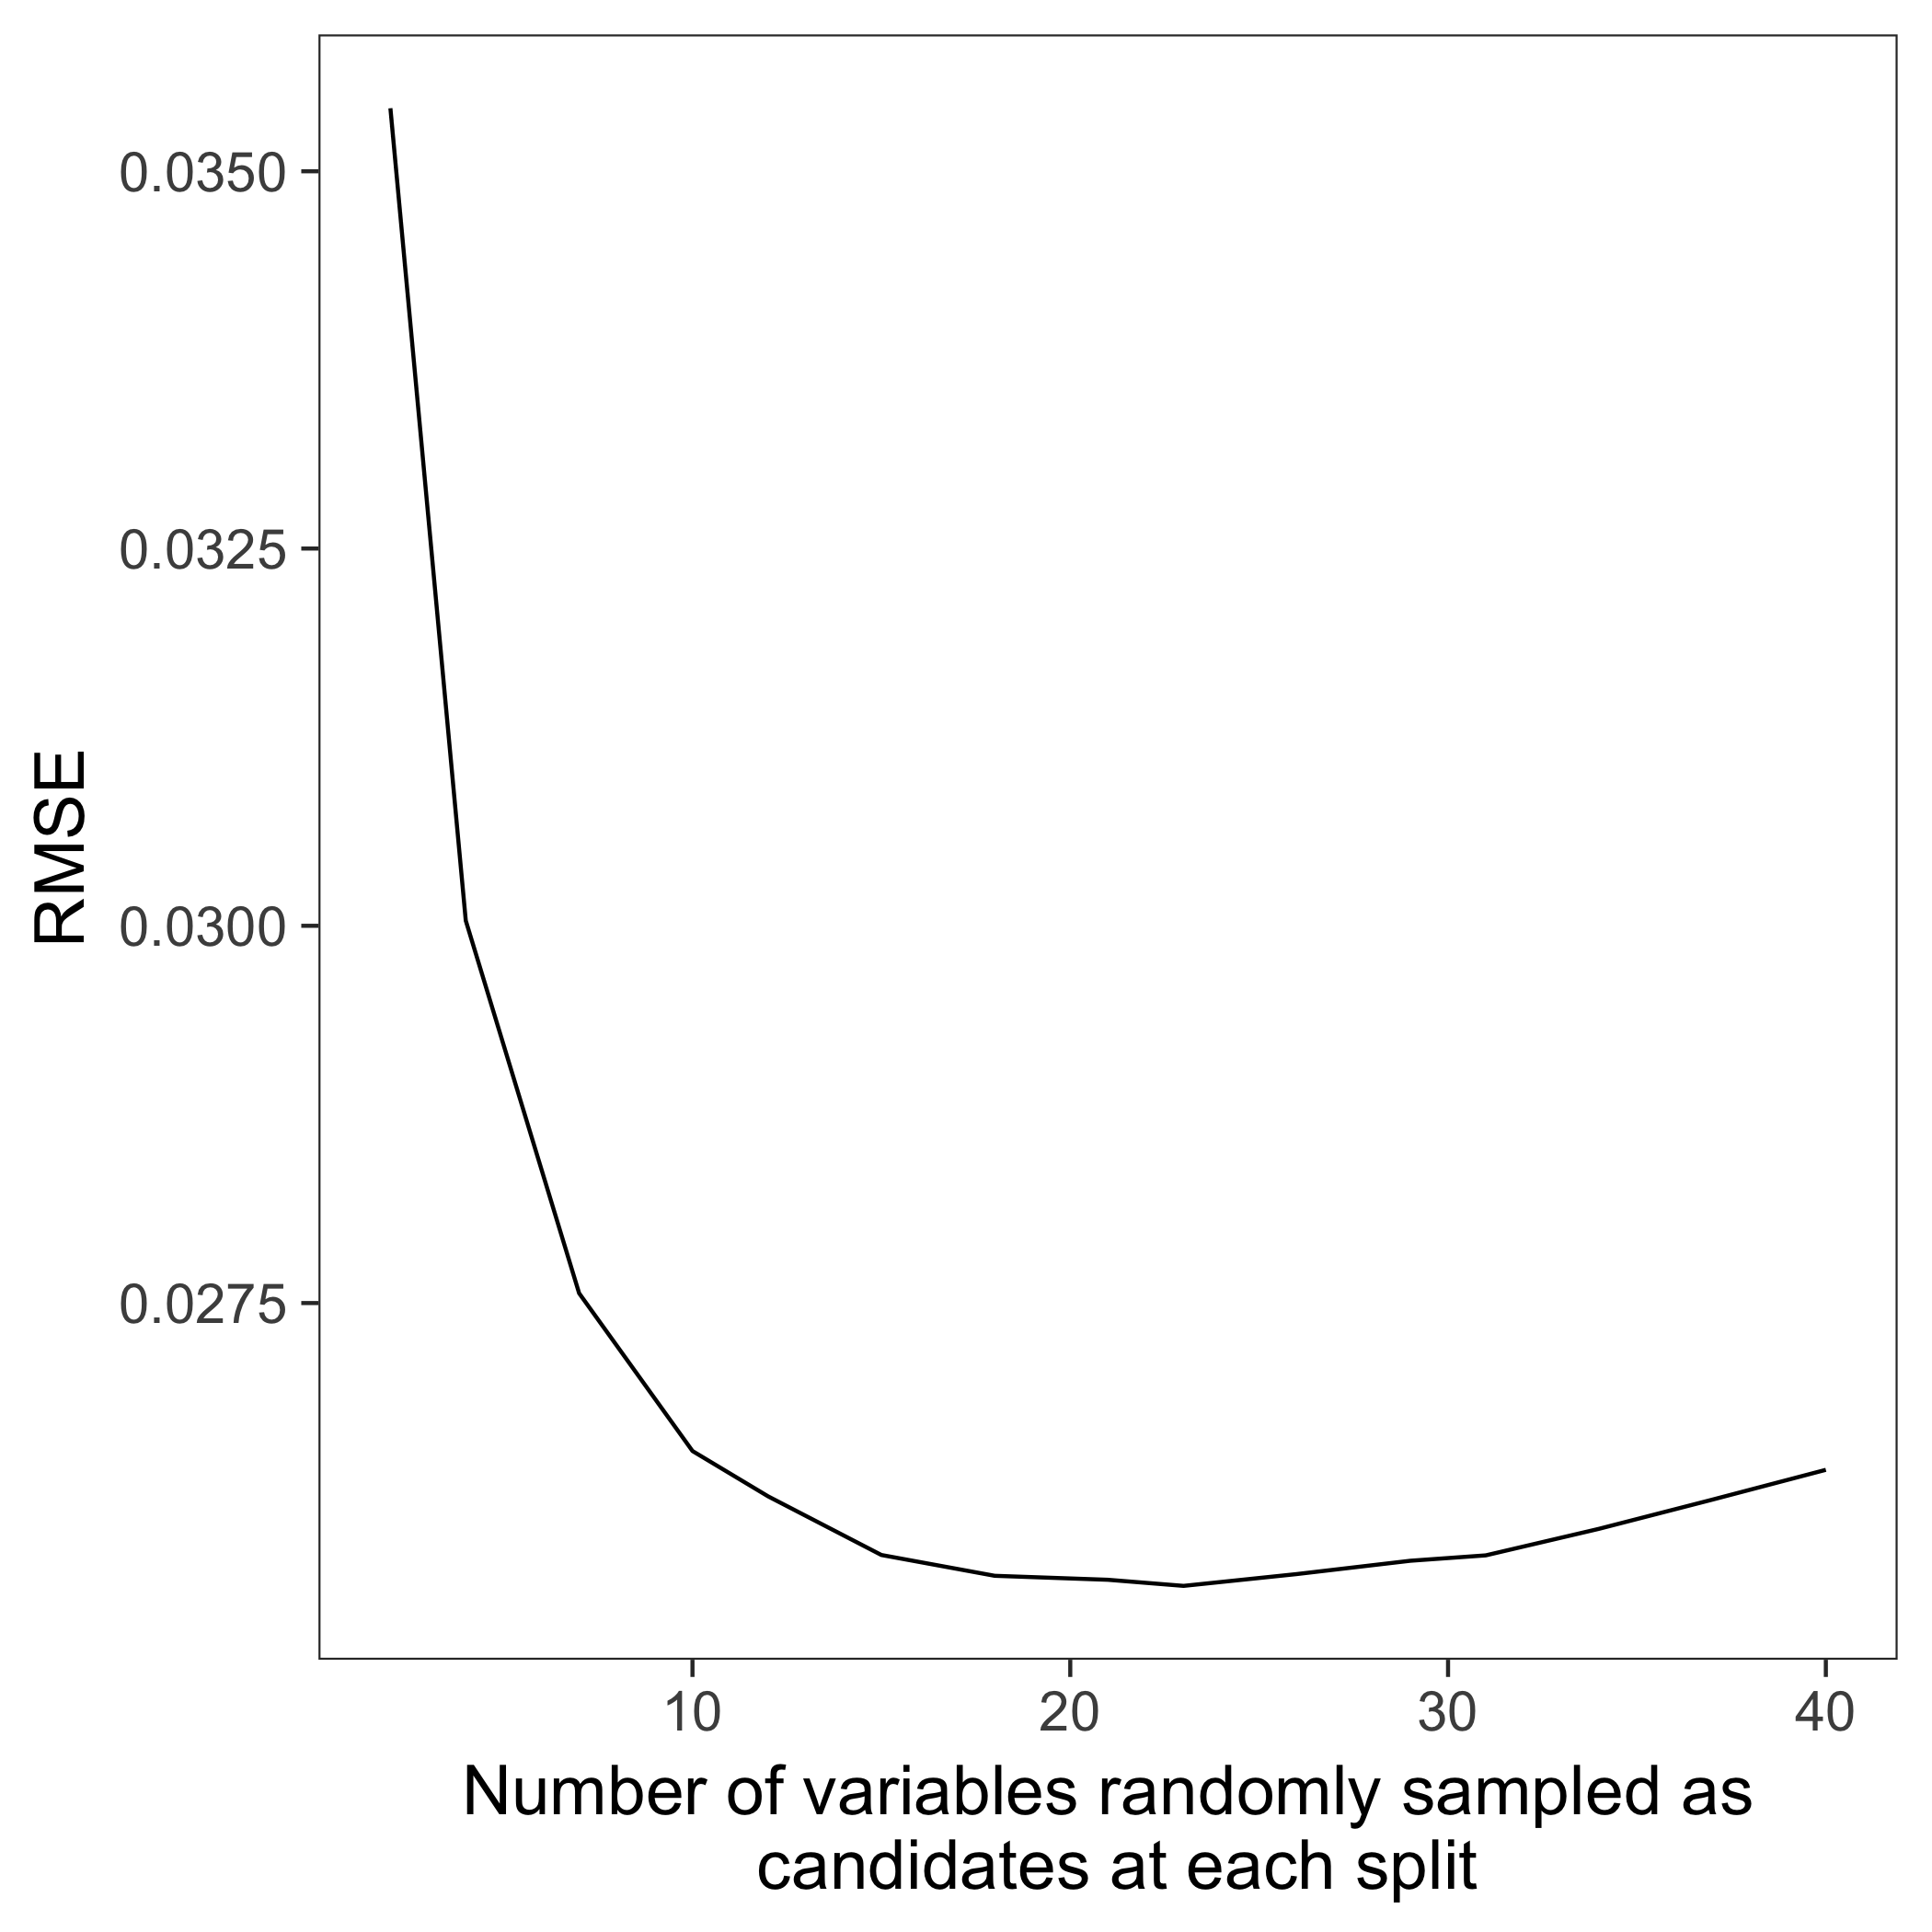
\includegraphics[width=0.8\textwidth]{Chapter5/figures/rforest_parameter_tuning}
	\caption{RMSE vs Number of variables randomly sampled as candidates at each split in the Random Forest model.}
	\label{fig:rf_param_tune}
\end{figure}

To initialize the Random Forest algorithm with the number of variables randomly sampled as candidates at each split, cross-validation was used. Once again, 75\% of the data was used for training and the remaining 25\% for testing due to the trade-off between training and testing.

Figure \ref{fig:rf_param_tune} shows the results of tuning the parameter of the number of variables randomly sampled as candidates at each split. The optimum number was found to be 23. Either side of this value the RMSE increases. Therefore the value 23 was selected to be the number of variables randomly sampled as candidates at each split in the Random Forest model. It is proposed that the value 23 was found to be optimum due to the 20 lagged inputs, as this data is crucial for the Random Forest to learn the underlying nature of electricity load.


\subsubsection{Multilayer Perceptron}

A feed-forward Multilayer Perceptron is a common neural network architecture used for the prediction of time series data, which has comparable, and occasionally better results than statistical models \cite{Hill1994}. 

The first step when designing a Multilayer Perceptron neural network is to design the architecture. For this case, the number of input neurons is set to 41 (see Table \ref{tab:feature}). Once an input for each neuron is entered, the output layer must be designed. Due to the fact that we are forecasting only one time step ahead (30 minutes ahead) one output neuron is required.

The next step is to design the architecture of the hidden layers. To accomplish this, cross-validation is utilised as per the previous models. A maximum of 3 hidden layers were tested and the results analysed. A similar method to Fan \textit{et al.} was evaluated to choose the number of neurons and hidden layers, a technique known as the Levenberg-Marquardt technique \cite{Fan2009}. The Levenberg-Marquardt is a technique suitable for training medium-sized Artificial Neural Networks with a low mean-squared error. 

The fundamental rule is to select the minimum number of neurons in the hidden layer so as to capture the complexity of the model, but not too many as to introduce over-fitting, which results in a loss in generalization of the algorithm.

The method begins by choosing a small number of neurons and gradually increasing the number each time the model is trained and the forecast error obtained. The forecast error is monitored until an optimum value is found, to which no further improvement is noted. Once the optimum number of neurons in the layer is obtained an additional layer is added, and the same technique is used.

Using this technique an optimal architecture with three layers is obtained. The first layer contained two neurons, the second contained five, and the third contained four.



\subsubsection{LSTM}

To initialize the LSTM, cross-validation was used to select the number of stacked layers and memory units. Similarly to the technique used for the Multilayer Perceptron, the Levenberg-Marquardt was used. The optimum number of layers was found to be 2, with a total of 50 memory units. Different combinations of layers and memory units displayed worse results.



\section{Results}


\begin{figure}
	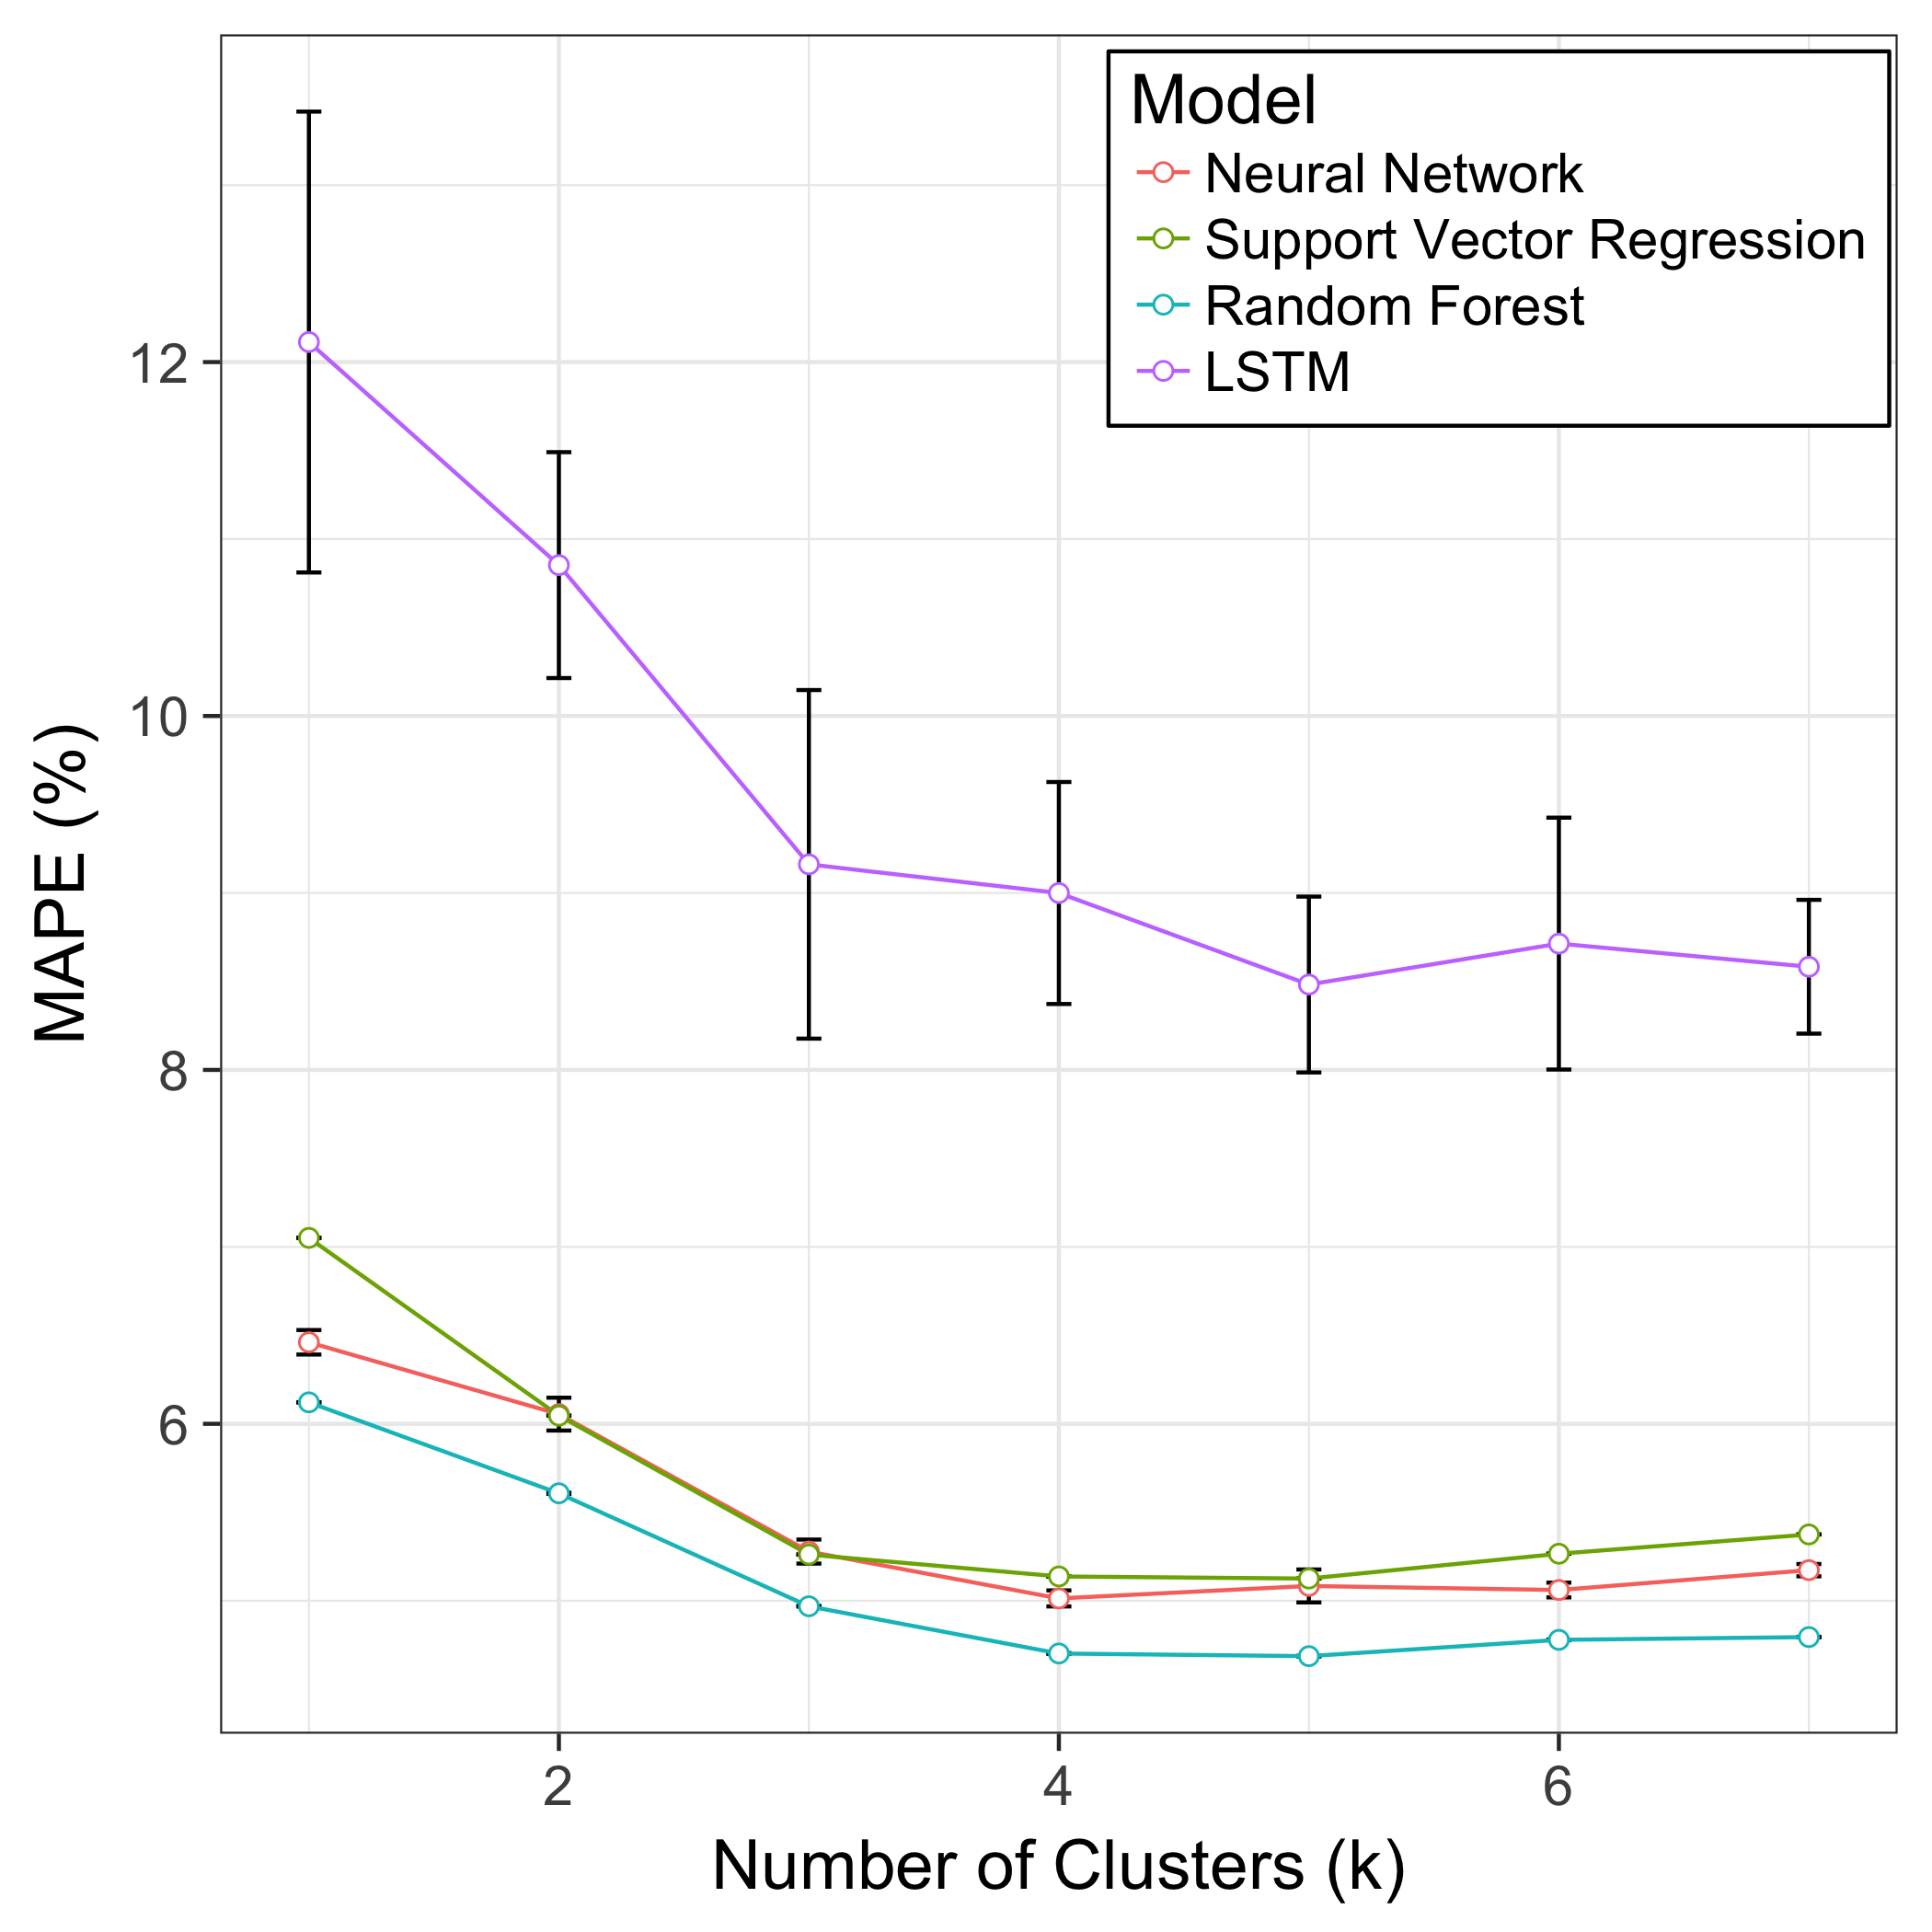
\includegraphics[width=0.8\textwidth]{Chapter5/figures/results.png}
	\caption{Comparison of accuracy of models forecasting electricity with varying number of clusters.}
	\label{fig:results}
\end{figure}

\begin{figure}
	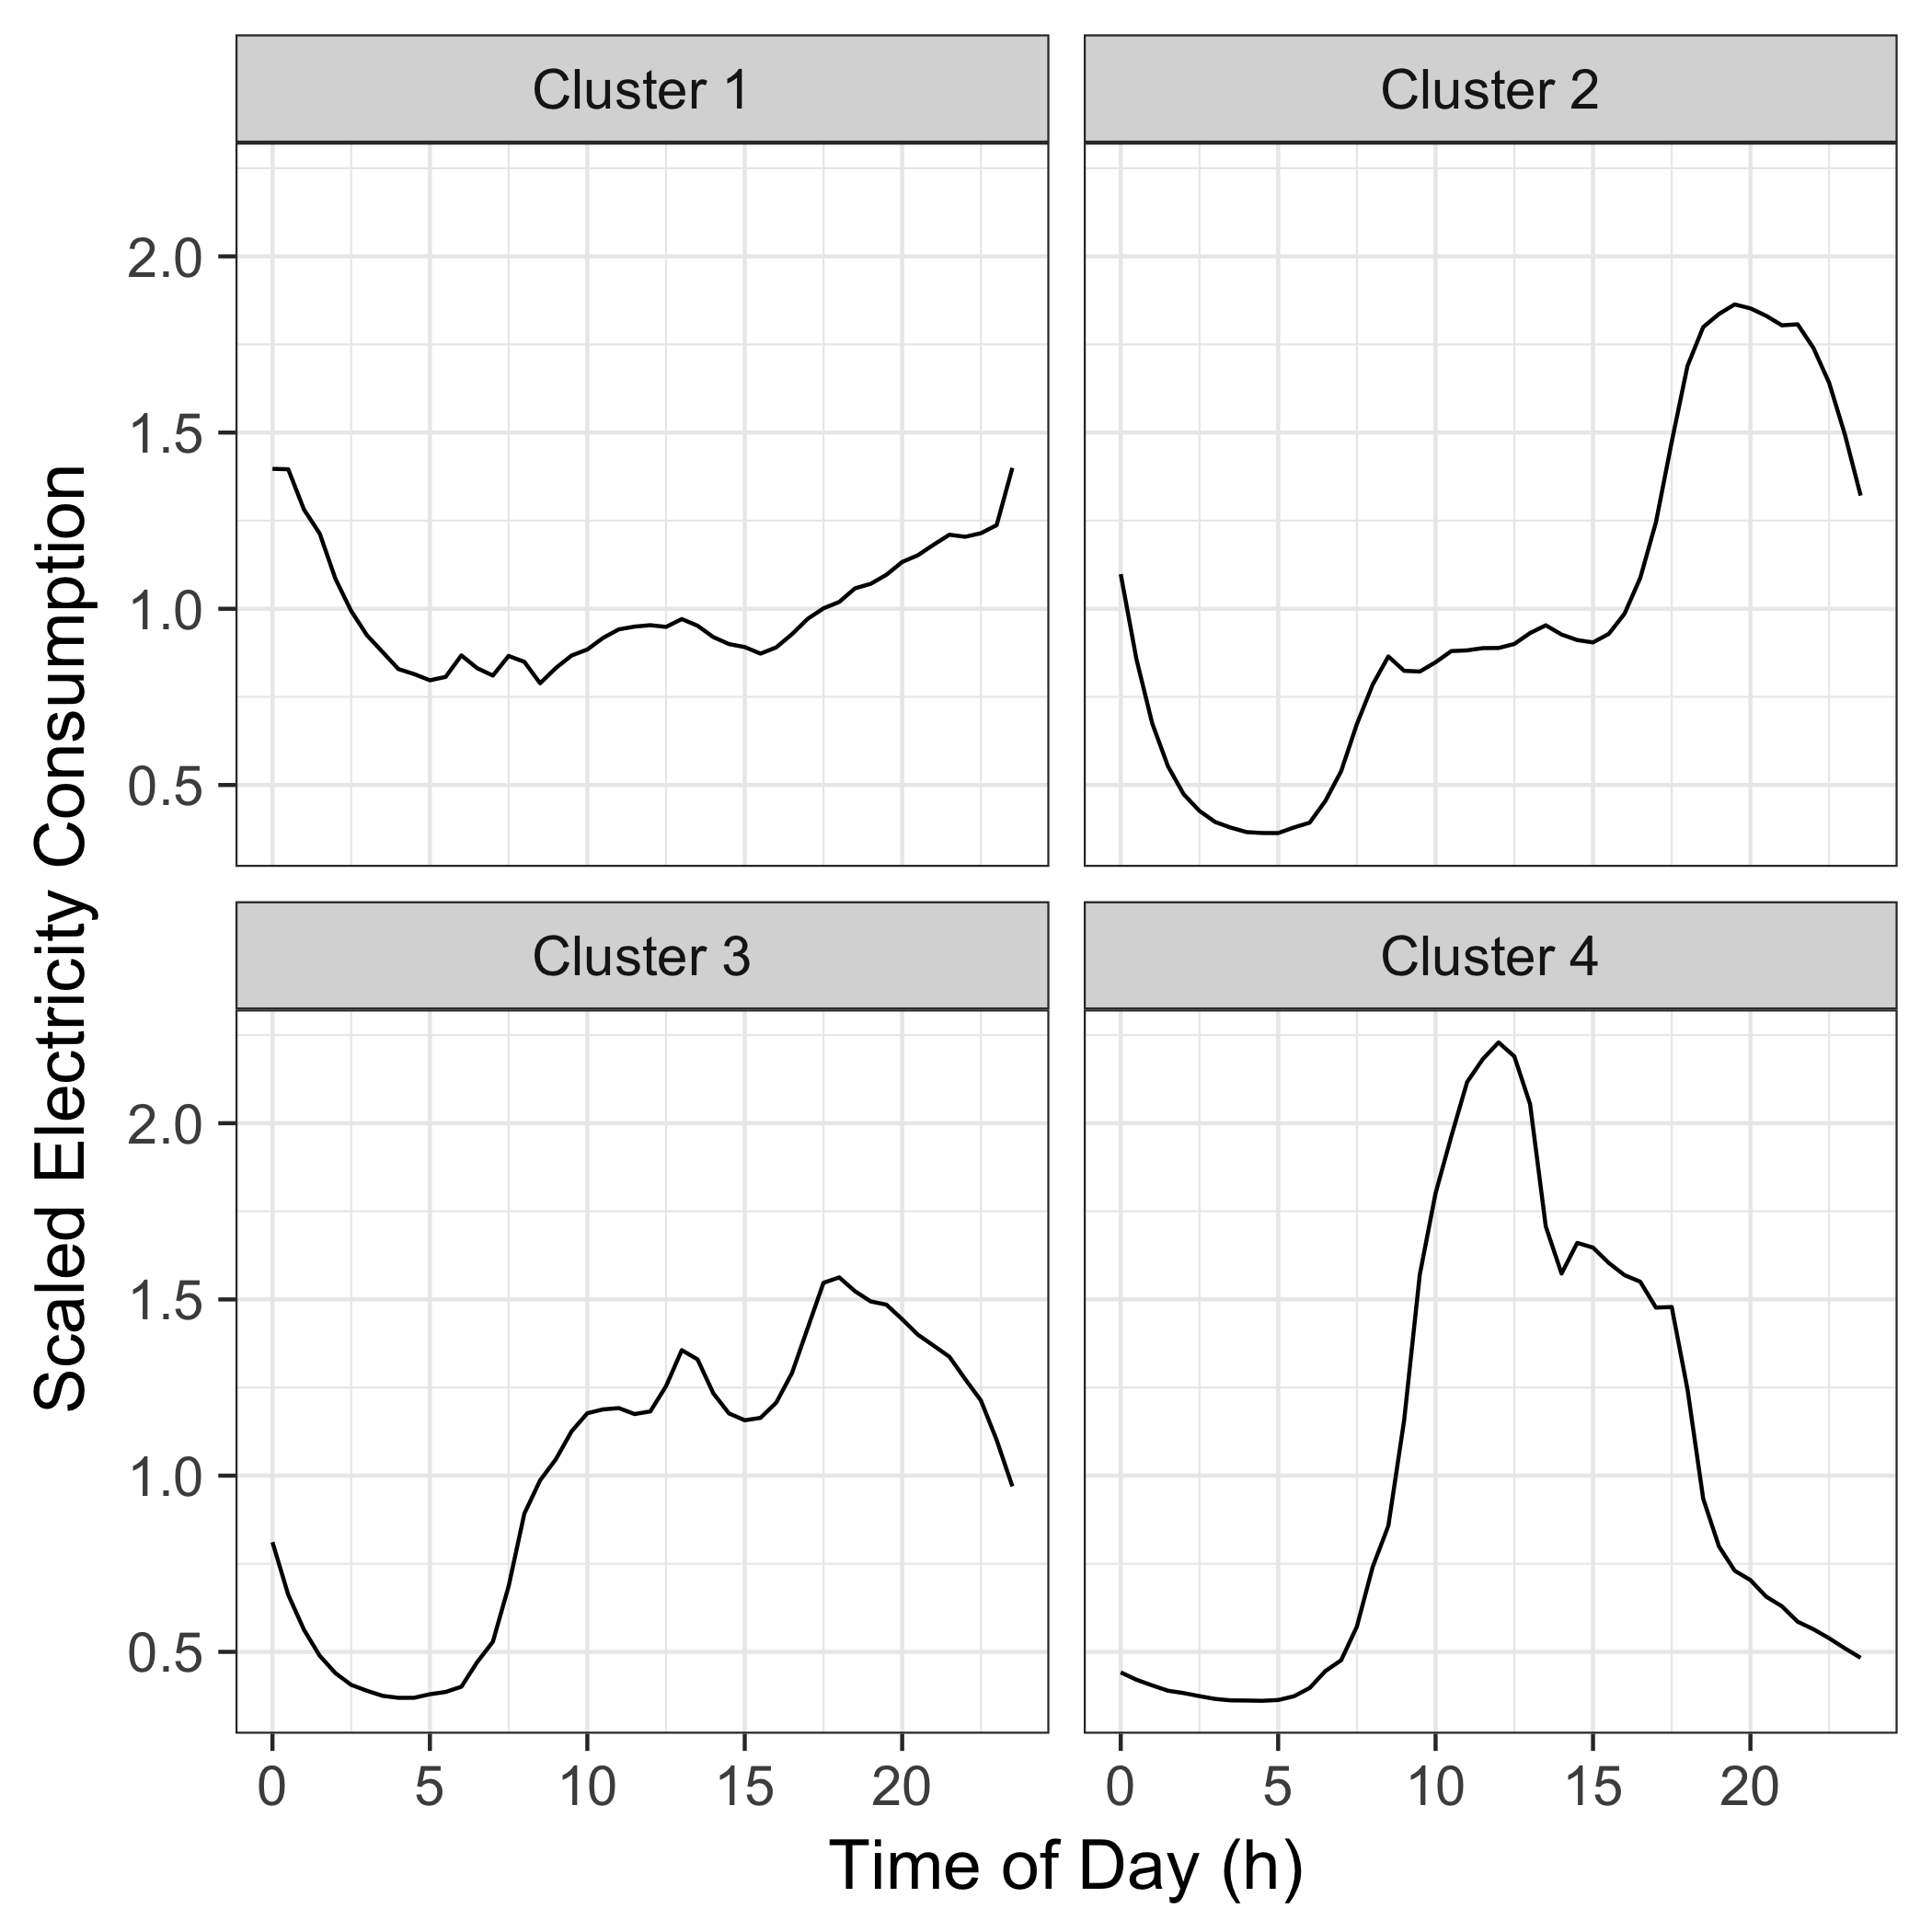
\includegraphics[width=0.8\textwidth]{Chapter5/figures/Cluster_Centres.png}
	\caption{Average load profile for each cluster.}
	\label{fig:clustercentre}
\end{figure}

To test the accuracy of the trained model the data was split into a training and test set. The data between the 14th of July 2009 and the 15th of June 2010 was used as the training data, whilst the data between the 15th of June 2010 and 31st of December 2010 was used for testing purposes. The test set is separate from the training set and not used during training. 

28 independent forecasting models are constructed for each of the Random Forests, Support Vector Regression, LSTMs and Multilayer Perceptron neural networks for each of the groups with \textit{k} varying from 1 to 7. This was done to determine the optimal number of clusters.  Each of the 28 models are trained independently, five times each so that the standard deviation results of MAPE for each cluster could be displayed. We evaluated the MAPE of the overall prediction. 

Figure \ref{fig:results} displays the accuracy of the models trained at different numbers of clusters (\textit{k}). The results demonstrate that introducing clusters to group similar customers improve results in all cases. The optimum value for \textit{k} for Random Forests, Support Vector Regression and neural networks was shown to be four for our dataset. After this, the accuracy diminishes slightly. The error bars shown in Figure \ref{fig:results} show a small variance in MAPE in SVRs, ANNs and Random Forests. However, the MAPE of the LSTMs seem to vary by up to 11\% in the five models run. 

Figure \ref{fig:calendar_attr} demonstrates the impact of using calendar attributes such as month, day of the month, and day of the week on prediction accuracy. The results show an increase in prediction accuracy of 6\% for neural networks, 4\% for Random Forests and 1\% for support vector regression when taking into account these variables. It is proposed that the ability for the models to take into account the cyclic yearly, monthly and weekly behaviour improves the results.

\begin{figure}
	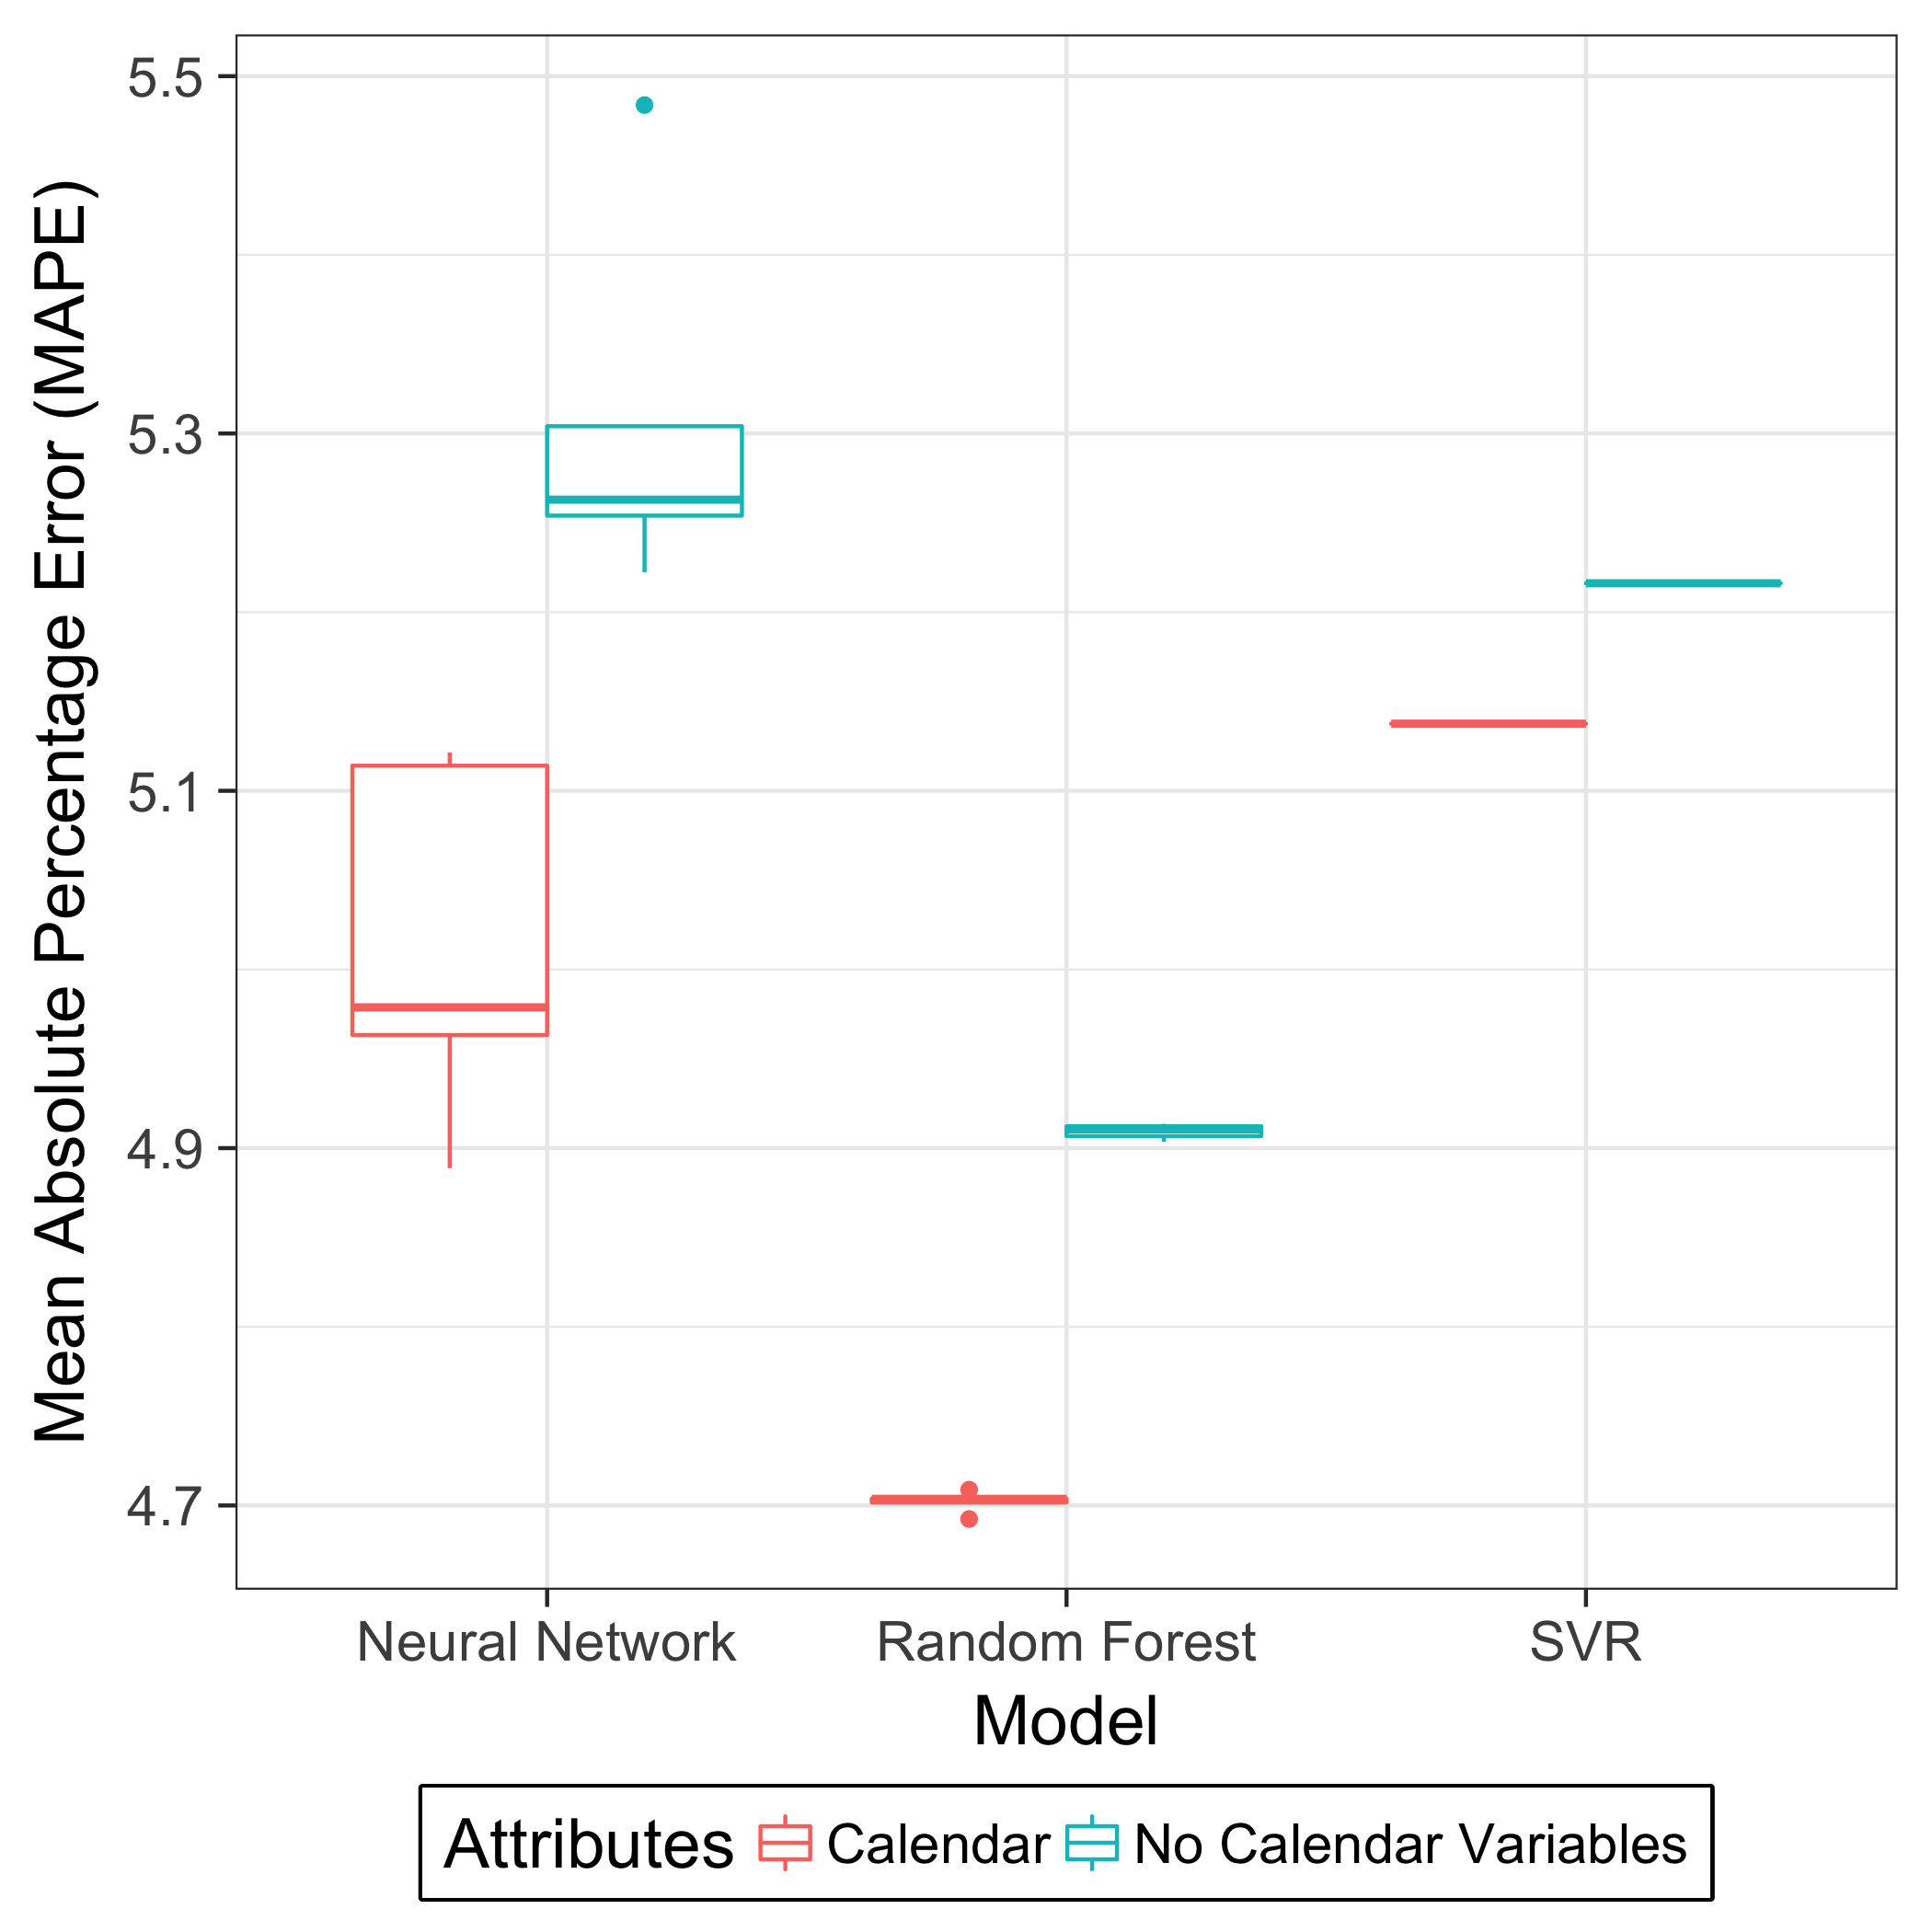
\includegraphics[width=0.8\textwidth]{Chapter5/figures/calendar_attr.png}
	\caption{Comparison of accuracy of models with or without calendar attributes.}
	\label{fig:calendar_attr}
\end{figure}



Figure \ref{fig:clustercentre} shows the average load profiles of different clusters when $k=4$. It is proposed that the optimum number of clusters is four due to the distinct load profiles that can be seen in Figure \ref{fig:clustercentre}. The four different distinct patterns seen are high night time use in cluster 1, a typical residential load profile is shown in cluster 2, a spread of usage in cluster 3, and high daytime usage in cluster 4. At $k=3$ these distinct patterns are not adequately clustered, and at $k=5$ one of the distinct clusters are split, leading to an increase in stochasticity.

It is true that the optimum number of clusters will vary for different datasets. Whilst residential smart meter datasets may be similar, it is entirely possible that different geographies display different usage characteristics based on factors such as culture, temperature and economical reasons. It is therefore important to choose an optimal number of clusters for each dataset.

The results demonstrate that SVR, Random Forests and the Multilayer Perceptrons have a similar overall accuracy. The LSTM shows a similar pattern in increasing accuracy with number of clusters. However, the Random Forest seems to outperform each of the models at every point. This may be due, in part, to the internal operation of the Random Forest which undertakes its own cross-validation using out-of-bag samples and only having a few tuning parameters. 

It has been shown that neural networks, SVR and Random Forests all perform within an adequate range of predicting electricity consumption. Whilst LSTMs perform poorly. This may be due to the features given to the LSTM which only had previous two and a half hours of data as input. 

However, it is well known that the best machine learning technique for predicting energy consumption cannot be chosen \textit{a priori}. Therefore it is necessary to compare different techniques to find the best solution to a particular regression problem \cite{Ahmad2017}.

For this work, the training time was tested by timing how long the models would be fit to create one cluster (single model trained on the training set). The Support Vector Regression took much less time than all of the other methods, whereas the LSTM took the longest. The Artificial Neural Network required 9 minutes and 5 seconds to run. The Support Vector Regression model required 3 minutes and 32 seconds to run. The Random Forest, on the same data, required 9 minutes and 44 seconds to run, whilst the LSTM took 12 minutes 55 seconds. 


\section{Conclusion}

The availability of high granularity data produced by the smart grid enables network operators to gain greater insights into their customer behaviour and electricity usage. This enables them to improve customer experience, utility operations and power management. We demonstrated that implementing the \textit{k}-means clustering algorithm to group similar customers improved the accuracy of every one of the different models tested. Distinct models were trained for each of the clusters and the individual forecasts aggregated for the total aggregated forecast. It was found that Random Forests outperformed  the other models at all levels of clustering and that the optimum number of clusters was 4. Whilst the dataset used focused on residential data it is expected that applying a similar clustering technique on commercial properties would have a similar effect.

In future work, we will look into the features that best aid in the forecasting of electricity consumption, try a wider variety of models in an ensemble manner and try different clustering techniques such as self-organizing maps (SOM) to obtain better accuracy measures. We will also compare different prediction error measures.

To utilize more of the data and increase the number of models trained these results could be run in parallel and on the cloud in future.



\section{Note paper}

\section{Introduction}

The energy markets have undergone significant changes in recent years. The liberalisation of the energy industry, technological advancements and policy changes have had numerous effects \cite{Viegas2016}. These include a rise in both competition and data \cite{sioshansi_2009, Clastres2011}. %, as well as a requirement to integrate large amounts of intermittent renewable resources \cite{Haben2013a,Kamgarpour2013,Curves2014}.

Accurate load forecasting is essential for control and planning of electricity generation in electrical grids as supply must meet demand \cite{Lu1993}. Accurate estimates of demand are required so that the correct amount of electricity is purchased on the wholesale market \cite{Dillon1991}. Failure to accurately forecast electricity demand can lead to financial loss or system-wide blackouts \cite{Hines2008}.

The introduction of smart meters in many countries (USA, Europe and South Korea) has led to an influx of high granularity electricity consumption data that can be used for load forecasting \cite{Depuru2011a}. 800 million smart meters are projected to be installed worldwide by 2020 \cite{Telefonica2014}. 

This paper explores short-term load-forecasting at an interval of 30 minutes ahead and clusters similar users based on their electricity consumption. A variety of different forecasting techniques were evaluated such as Random Forests \cite{TinKamHo}, Long Short-Term Memory Neural Networks (LSTM) \cite{lstm}, Artificial Neural Networks \cite{book:984557} (ANN) and Support Vector Regression (SVR) \cite{Drucker1997}. 

Random Forests are an ensemble-based learning method for classification and regression, and are made up of many decision trees. LSTMs are recurrent Neural Networks which remember values over arbitrary time intervals. Multilayer Perceptrons are a popular type of neural network which consist of a minimum of three layers and can be used to make non-linear predictions. SVRs are supervised learning models which analyse data for regression analysis.

To improve forecasting results, \textit{k}-means clustering of smart meter data was evaluated. An average 24-hour electricity load profile per customer was calculated, and the result used for clustering. The clustered sub-system is then aggregated and separate models trained on these aggregates. The yearly, weekly and daily periodicity of electricity load is accounted for by feature vectors. Once forecasts for each cluster are made using the individual models, the results are aggregated for the final predictions. These predictions are compared to the actual results and the accuracy measured using mean absolute percentage error (MAPE) and mean absolute scaled error (MASE).

This paper provides researchers and utilities with methods to maximise forecasting accuracy through the selection of machine learning and clustering algorithms.

This paper is structured as follows. In Section 2 we explore related work of load forecasting. The experiments and their evaluation are discussed in Section 3. The results are discussed in Section 4. In Section 5 we conclude and consider future directions for this work.

\section{Related Work}

The forecasting of aggregated and clustered electricity demand has been the focus of a considerable amount of research in recent years. The research can generally be classified into two classes, Artificial Intelligence (AI) techniques \cite{Kim2000, Tiong2008,Quilumba2014} and classical time series approaches \cite{Nazarko2005ARIMAApproach,Huang2003,Nguyen2017}. For the purposes of our paper we have reviewed artificial intelligence techniques. Please refer to appendix \ref{appendix:time_series} to explore the literature related to classical time series approaches.

Singh \textit{et al.} produced a review of load forecasting techniques and methodologies and reported that hybrid methods, which combine two or more different techniques, are gaining traction, as well as soft computing approaches (AI) such as genetic algorithms \cite{Singh2012}.

\subsection{Artificial Intelligence Techniques}

Dillon \textit{et al.} presented a Neural Network for short-term load forecasting. Their Neural Network consisted of three-layers and used adaptive learning for training \cite{Dillon1991}. They proposed the use of weather information to augment their electricity load data. They found better results with the Adaptive Neural Network than with a linear model, or Non-Adaptive Neural Network. In contrast to Dillon our paper focuses on a Non-Adaptive Neural Network and does not take into account weather information.

Chen \textit{et al.} used an Artificial Neural Network to predict electricity demand of three substations in Taiwan. They integrated temperature data into the model, and showed a higher degree of accuracy when forecasting demand in residential and commercial substations as opposed to industrial. This was due to the ability to model the high usage of air-conditioners in residential and commercial substations using temperature data \cite{Chen1996}. In contrast to the work by Chen \textit{et al.}, we focus on client-side prediction using smart meter data. We were, therefore, able to cluster the data based on load profile, as opposed to grouping based on geographical location.


\subsection{Clustering}

Multiple techniques have been proposed for the clustering of electricity load data prior to forecasting. Shu \textit{et al.} and Nagi \textit{et al.} propose a hybrid approach in which self-organizing maps are used to cluster the data, and Support Vector Regression is used for prediction \cite{Shu2006, Tiong2008}. This technique proved robust for different data types. Shu showed that this hybrid approach out-performed a single SVR technique, whilst Nagi showed superior results to a traditional ANN system. In contrast to both Nagi \textit{et al.} and Shu \textit{et al.} our paper utilises \textit{k}-means as the clustering algorithm.

Wijaya \textit{et al.} demonstrated that implementing  a certain number of clusters improved load-forecasting accuracy \cite{Wijaya2010}. However, a study by Ili\'c \textit{et al.}, showed that increasing the number of clusters did not improve accuracy \cite{Ilic2013}.

\section{Methodology}

The work in this paper was run on a MacBook Pro with a quad-core 3.1GHz Intel Core i7 processor with 16 GB 1867 MHz DDR3 of RAM and a 500GB solid state drive (SSD).

\subsection{Data Collection}

Smart meter data obtained from the Irish Social Science Data Archive (ISSDA) was used in this study \cite{cer_2012}. The Commission for Energy Regulation released a public dataset of anonymised smart meter data from the "\textit{Electricity Smart Metering Customer Behaviour Trials}" \cite{setis}. This dataset is made up of over 5000 Irish homes and businesses and is sampled at 30-minute intervals.

The data was recorded between the 14th July 2009 and 31st December 2010. For the purposes of cross-validation this data was split into a training, validation, and testing set. The training set consisted of the first 9 months of data and used to train the models, the validation set consisted of the following 2 months of data and used to tune the hyperparameters, and the test set included the remaining 6 months and used for measuring error. These splits were chosen to balance the training data with the test data and give the models a chance to learn the periodicity inherent in a one year period. Due to the long training times for these algorithms, we worked with a sample of 709 individual Irish homes. However, due to the infrequent requirement to train these models, we believe our technique would be suited for the real life application.

Figure \ref{fig:similar_customers} displays four residential customer daily load profiles. It can be seen that whilst Customer 1 and Customer 2 have similar load profiles, Customer 3 and Customer 4 have significantly different load profiles.  This demonstrates that, whilst electricity consumption changes per-person, it is possible to cluster similar customers by their load profiles.
\begin{figure}[b]
	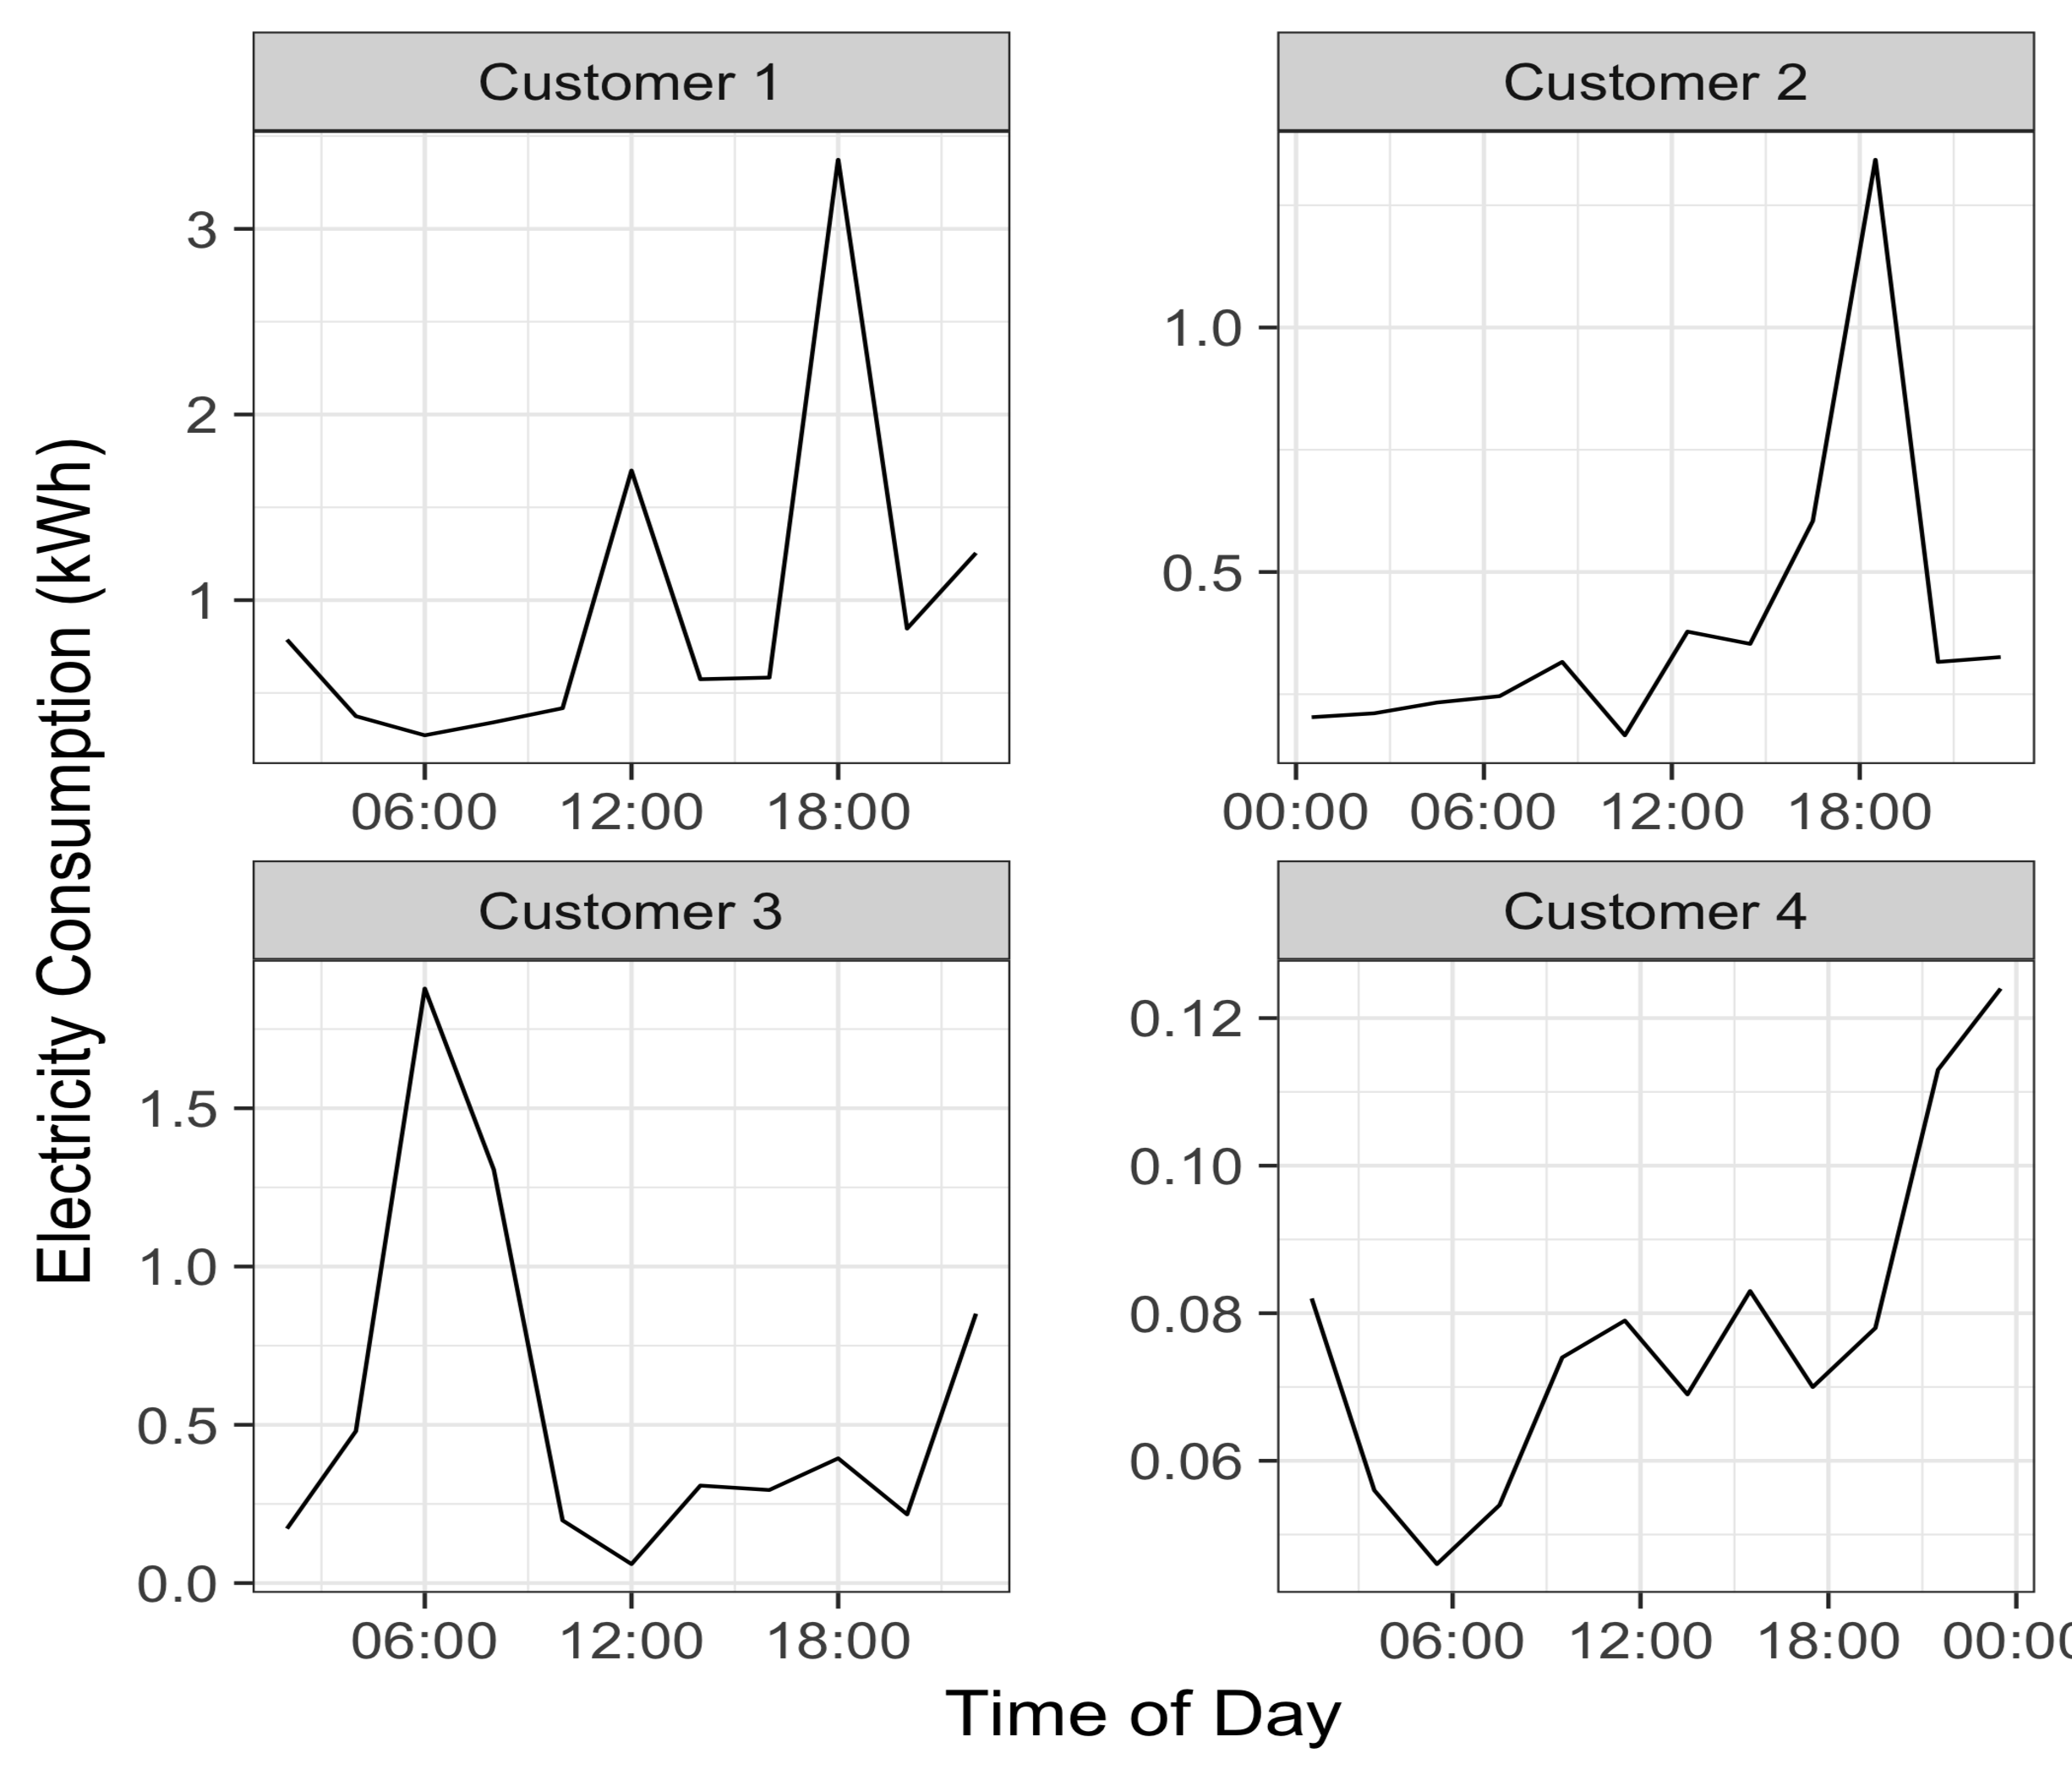
\includegraphics[width=0.8\textwidth]{Chapter5/figures/Webp_net-resizeimage.png}
	\caption{Figure showing daily load profiles for four different customers on the 22nd July 2009.}
	\label{fig:similar_customers}
\end{figure}
\subsection{Clustering}

We propose that clustering similar customer load profiles and aggregating each cluster's electricity consumption improves the accuracy of the models. This is due to the fact that aggregated clustered loads decrease the stochasticity of the demand of the system, and therefore increase the predictive ability of the models.

The Euclidean distance and wavelet metrics were evaluated using hierarchical clustering~\cite{BIMJ:BIMJ4710240520}. However, \textit{k}-means demonstrated to be the most robust and best-performing algorithm, and thus was chosen for use in this paper \cite{Forgy65}.

To cluster the data, each user's nine month electricity consumption in the training set was reduced to a single averaged 24 hour load profile (48 data points per customer). This was achieved by taking the average electricity consumed for each half hourly point of the day (eg. taking the mean of every 12-12:30pm point in the training set). We did not take into account the difference between weekend and weekdays for clustering. The data was then scaled so that different sized households, but with similar usage profiles were clustered together.

To select the optimum number of clusters (\textit{k}) the test set was used for cross-validation. This allowed us to compare the results of each of the models and select \textit{k} with the highest accuracy exhibited by mean absolute percentage error (MAPE) and mean absolute scaled error (MASE). In this paper \textit{k} was varied between 1 and 7, which was chosen due to the fact that the error did not vary greatly past seven clusters. Multiple models were fit per cluster and used to predict the testing data.

To overcome local minima the \textit{k}-means algorithm was run 1000 times and the most accurate partition chosen \cite{Jain2010}.

\subsection{Aggregating Demand}

Once each customer is assigned to their respective cluster, the total electricity consumed by each cluster is calculated. This is achieved by summing the electricity consumed at every time interval per cluster. This creates a partial system load. A model is trained on each of the different partial system loads, and the resultant forecasts are aggregated to generate the total load forecast. This forecast is then evaluated by calculating the MAPE and MASE for each model. 

\subsection{Feature Selection}

\subsubsection{Calendar Attributes}

Due to the daily, weekly and annual periodicity of the electricity consumption, daily calendar attributes were deemed important to accurately model the problem. The calendar attributes included are: hour of the day, day of the month, day of the week, month, and public holidays.

Public holidays were used as features for the model due to the change in electricity consumption exhibited on these days.

We evaluate the increase in performance due to the modelling of calendar attributes in the results section.

\subsubsection{Time Series Data}

The time-series element was modelled using lagged data inputs. This was achieved using the previous 3 hours, the equivalent 3 hours from the previous day, and the equivalent 3 hours from the previous week.

Long Short-Term Memory neural networks remember values over arbitrary time intervals. And thus can remember short-term memory over a long period of time, for this reason, 5 lagged inputs of the previous two and a half hours were used as features to the Long Short-Term Memory network.

\subsubsection{Data Representation}

Numerical representations were used for the lagged data input. A single binary was used for public holidays. One hot encoding is a method which allows categorical variables to be distinguished from ordinal data. One hot encoding was used to encode day of the week and month of the year. Table \ref{appendix:feature} displays the input data for SVR, Neural Network and Random Forest. 



\begin{table}
	\caption{List of Input Data for Models}
	\label{appendix:feature}
	\begin{tabular}{p{1cm}p{1.8cm}p{4.8cm}}
		\toprule
		Input & Variable      & Detail description \\
		\midrule
		1     & Hour          & Single numeric input representing hour of the day                                                                                              \\
		2     & Day of month  & Single numeric input representing day of the month                                                                                             \\
		3-9   & Day of week   & Seven binary digits representing calendar information regarding day of the week                                                                                            \\
		10-21 & Month         & Twelve binary digits representing calendar information regarding month                                                                                         \\
		22-42 & Lagged inputs & Twenty one numeric inputs representing lagged inputs of previous 3 hours, previous 3 hours of previous day including hour to be predicted, and previous 3 hours of previous week including hour to be predicted \\
		43    & Holiday       & Single binary digit representing whether the day was a public holiday  \\     \bottomrule                                                           
	\end{tabular}
\end{table}

\subsection{Experiments}

This section explores the experiments made to design the models. Cross-validation was used on the validation set of each of the models to tune the hyperparameters. Each of the models were then created five times per cluster to explore the variance of the results.

\subsubsection{Support Vector Regression}

The validation set was used to tune the hyperparameters and select the kernel of the SVR model.

The kernels compared were polynomial, radial basis function (RBF) and the linear kernel \cite{Chang2010, theodoridis2009pattern}. They were chosen due to their popularity, support and speed of computation.

The parameter values are shown in Table \ref{tab:kernel}. The linear kernel produced the best results, and therefore chosen as the final model.
\begin{table}
	\caption{Prediction Accuracy Based on Type of Kernel}
	\label{tab:kernel}
	\begin{tabular}{ccl}
		\toprule
		Kernel Type& Kernel Parameters & RMSE\\
		\midrule
		Linear & No values & 0.02102779\\
		RBF & C=2, $\gamma=0.016$ & 0.02444950\\
		Polynomial & C=2, $d=2, r=2$ & 0.03145719 \\
		\bottomrule
	\end{tabular}
\end{table}
\subsubsection{Random Forest}
The number of variables sampled as candidates at each split was tuned using the validation set.

The optimum number for this was 23. It is proposed that the value 23 was found to be optimum due to the 21 lagged inputs, which are crucial to learn the underlying nature of the time series.


\subsubsection{Artificial Neural Network}

The first step when creating an Artificial Neural Network is to design the architecture. In our case, the number of input neurons is set to 43 (see Table \ref{appendix:feature}). Only one output neuron is required, due to the fact that we are only forecasting one step (30 minutes) ahead.

To design the number of hidden layers the Levenberg-Marquardt technique was used. An optimal architecture with three hidden layers was obtained. The first layer contained two neurons, the second contained five, and the third contained four.

\subsubsection{LSTM}

The Levenberg-Marquardt techniques was once again used to select number of layers and number of memory units. Using this technique, the optimum number of layers was found to be 2 with 50 memory units each.

\section{Results}
\begin{figure}
	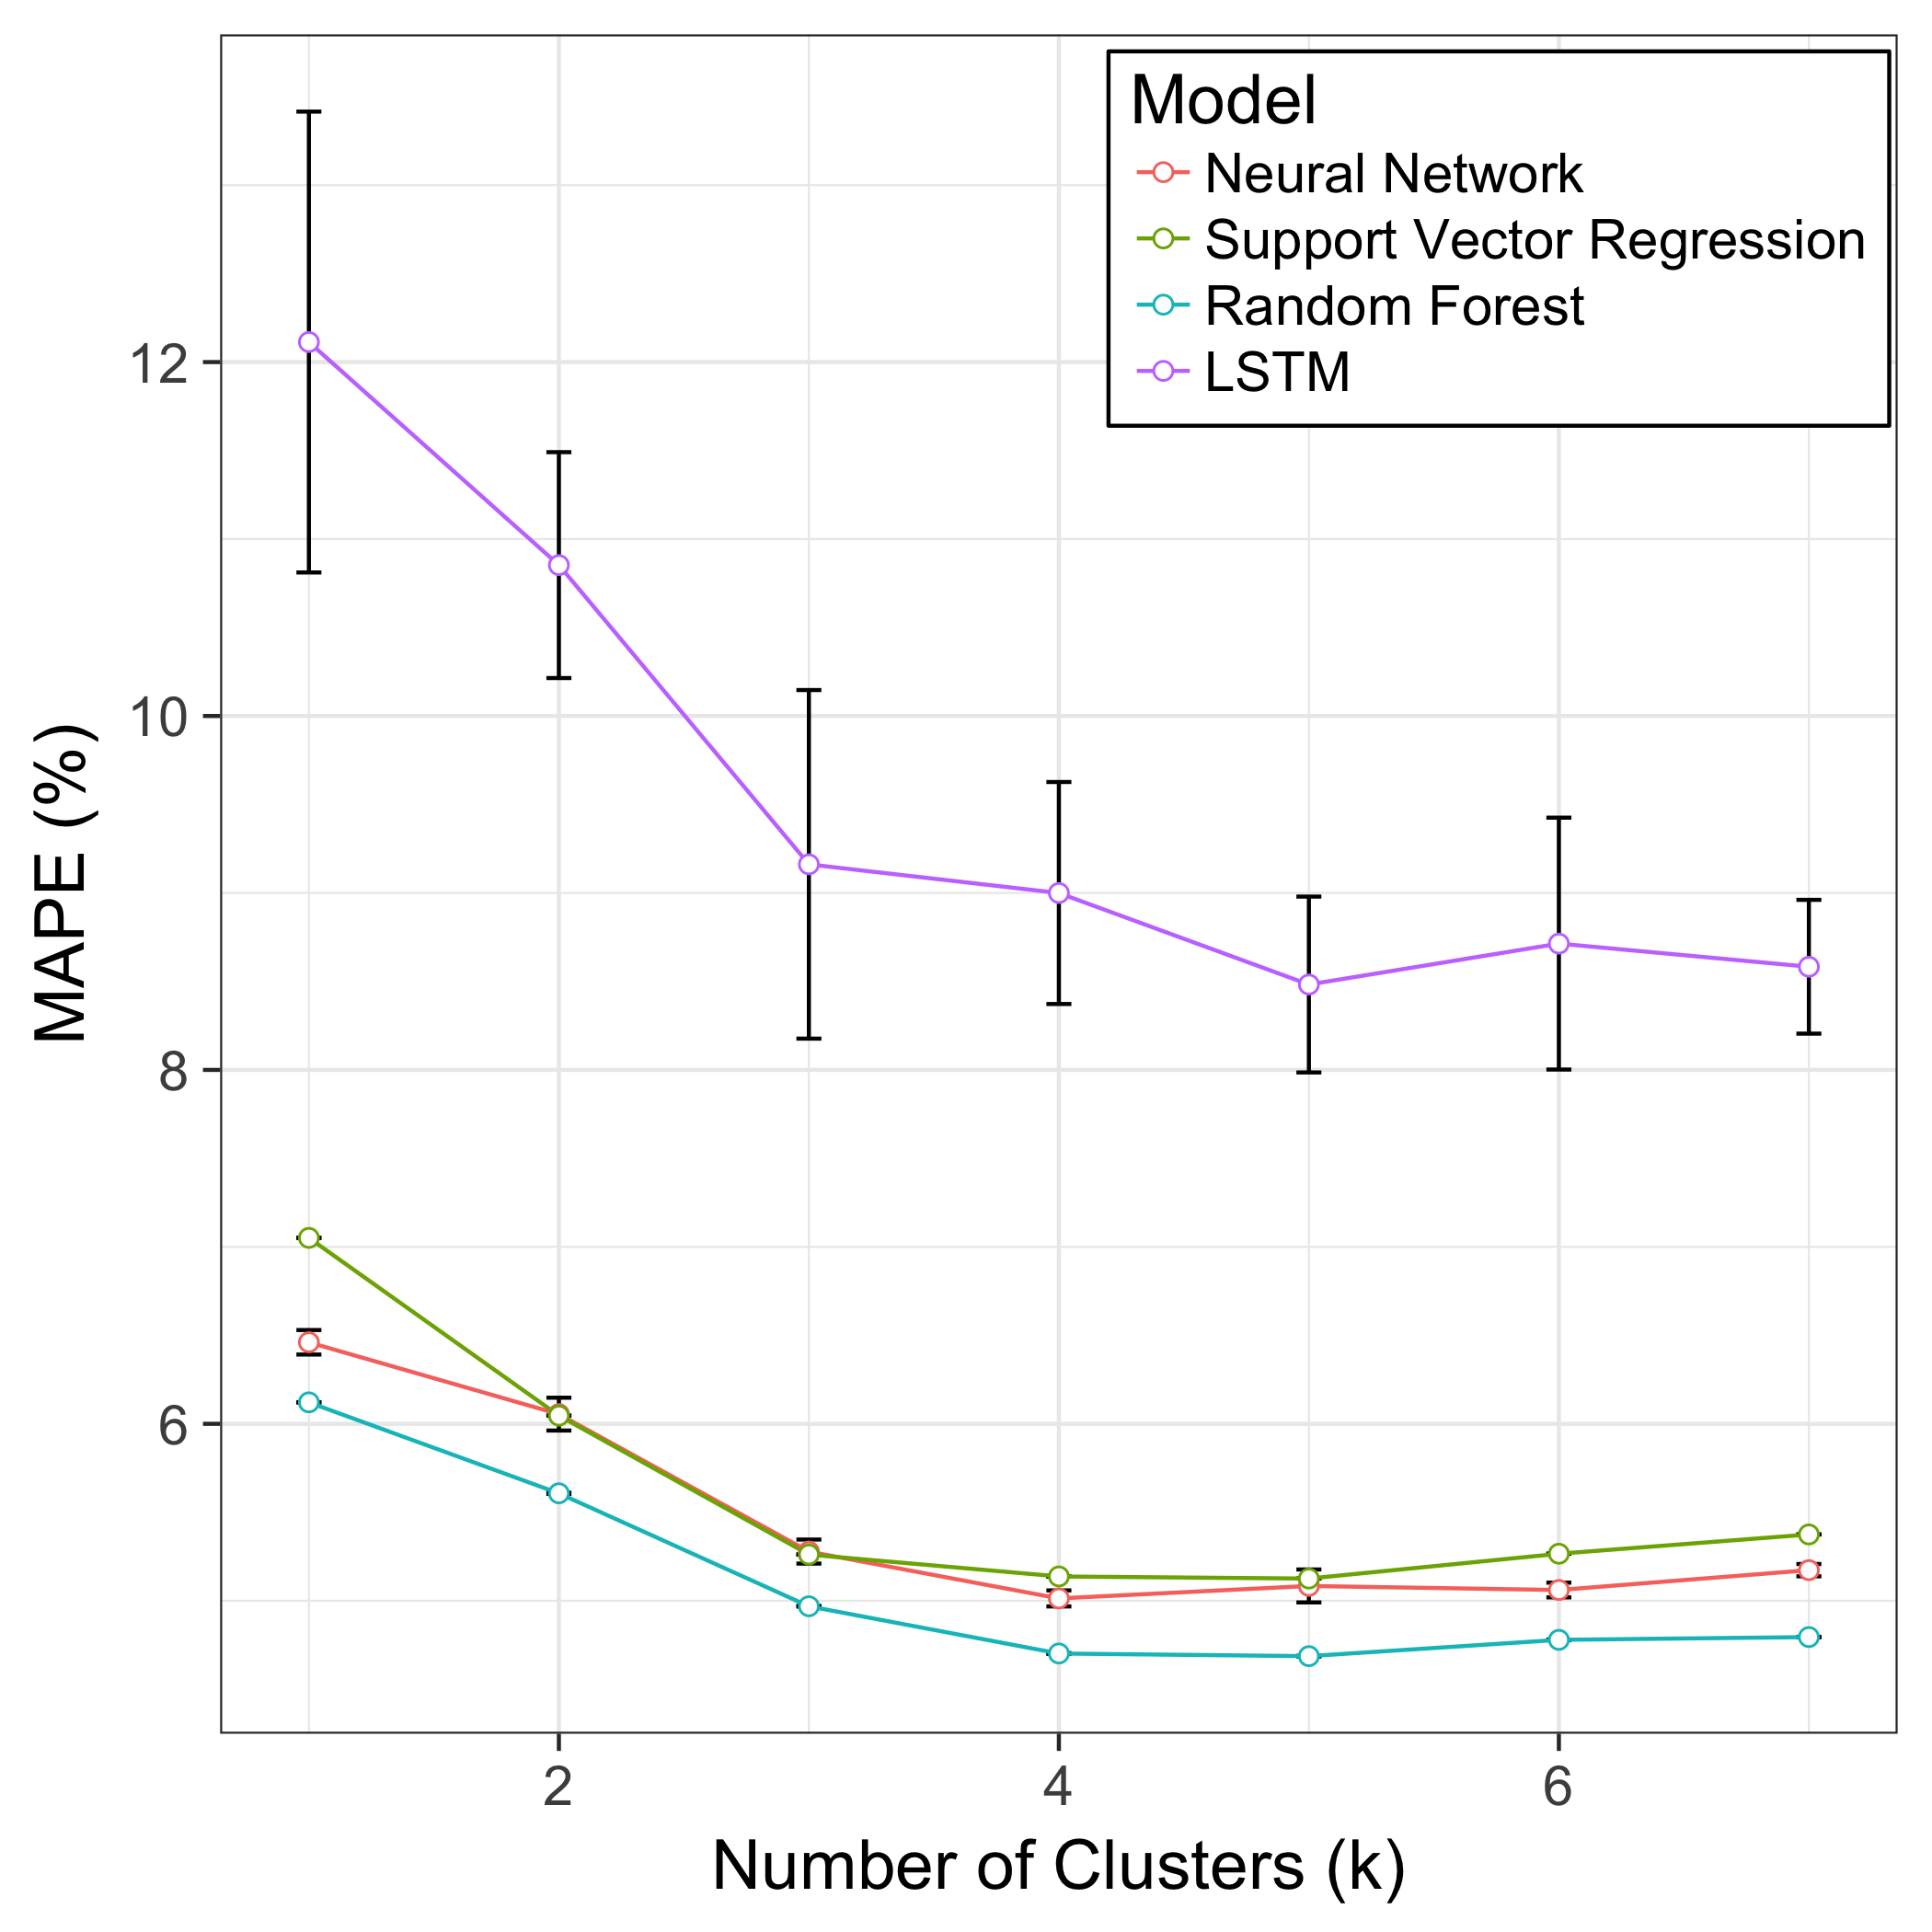
\includegraphics[width=0.8\textwidth]{Chapter5/figures/results.png}
	\caption{Comparison of accuracy of models forecasting electricity with varying number of clusters.}
	\label{fig:results}
\end{figure}
To determine the optimal number of clusters a range of values for $k$ were explored, thus, $k$ was varied between one and seven. 28 forecasting models were therefore constructed per type of model. The models were fit five times to explore the variation in the output. The model accuracy was evaluated using both MAPE and MASE.

The results are shown in figure \ref{fig:results}. These show that clustering similar users improves accuracy. The optimum value for \textit{k} for every model was shown to be four. After this, the accuracy diminishes slightly. The error bars shown in Figure \ref{fig:results} display a slight variance in MAPE for SVRs, ANNs and Random Forests. However, the MAPE of the LSTMs seem to vary by up to 11\%. 

The MASE metric also demonstrated that four clusters were optimal for SVR, Neural Networks and Random Forests.

\begin{figure}
	\centering
	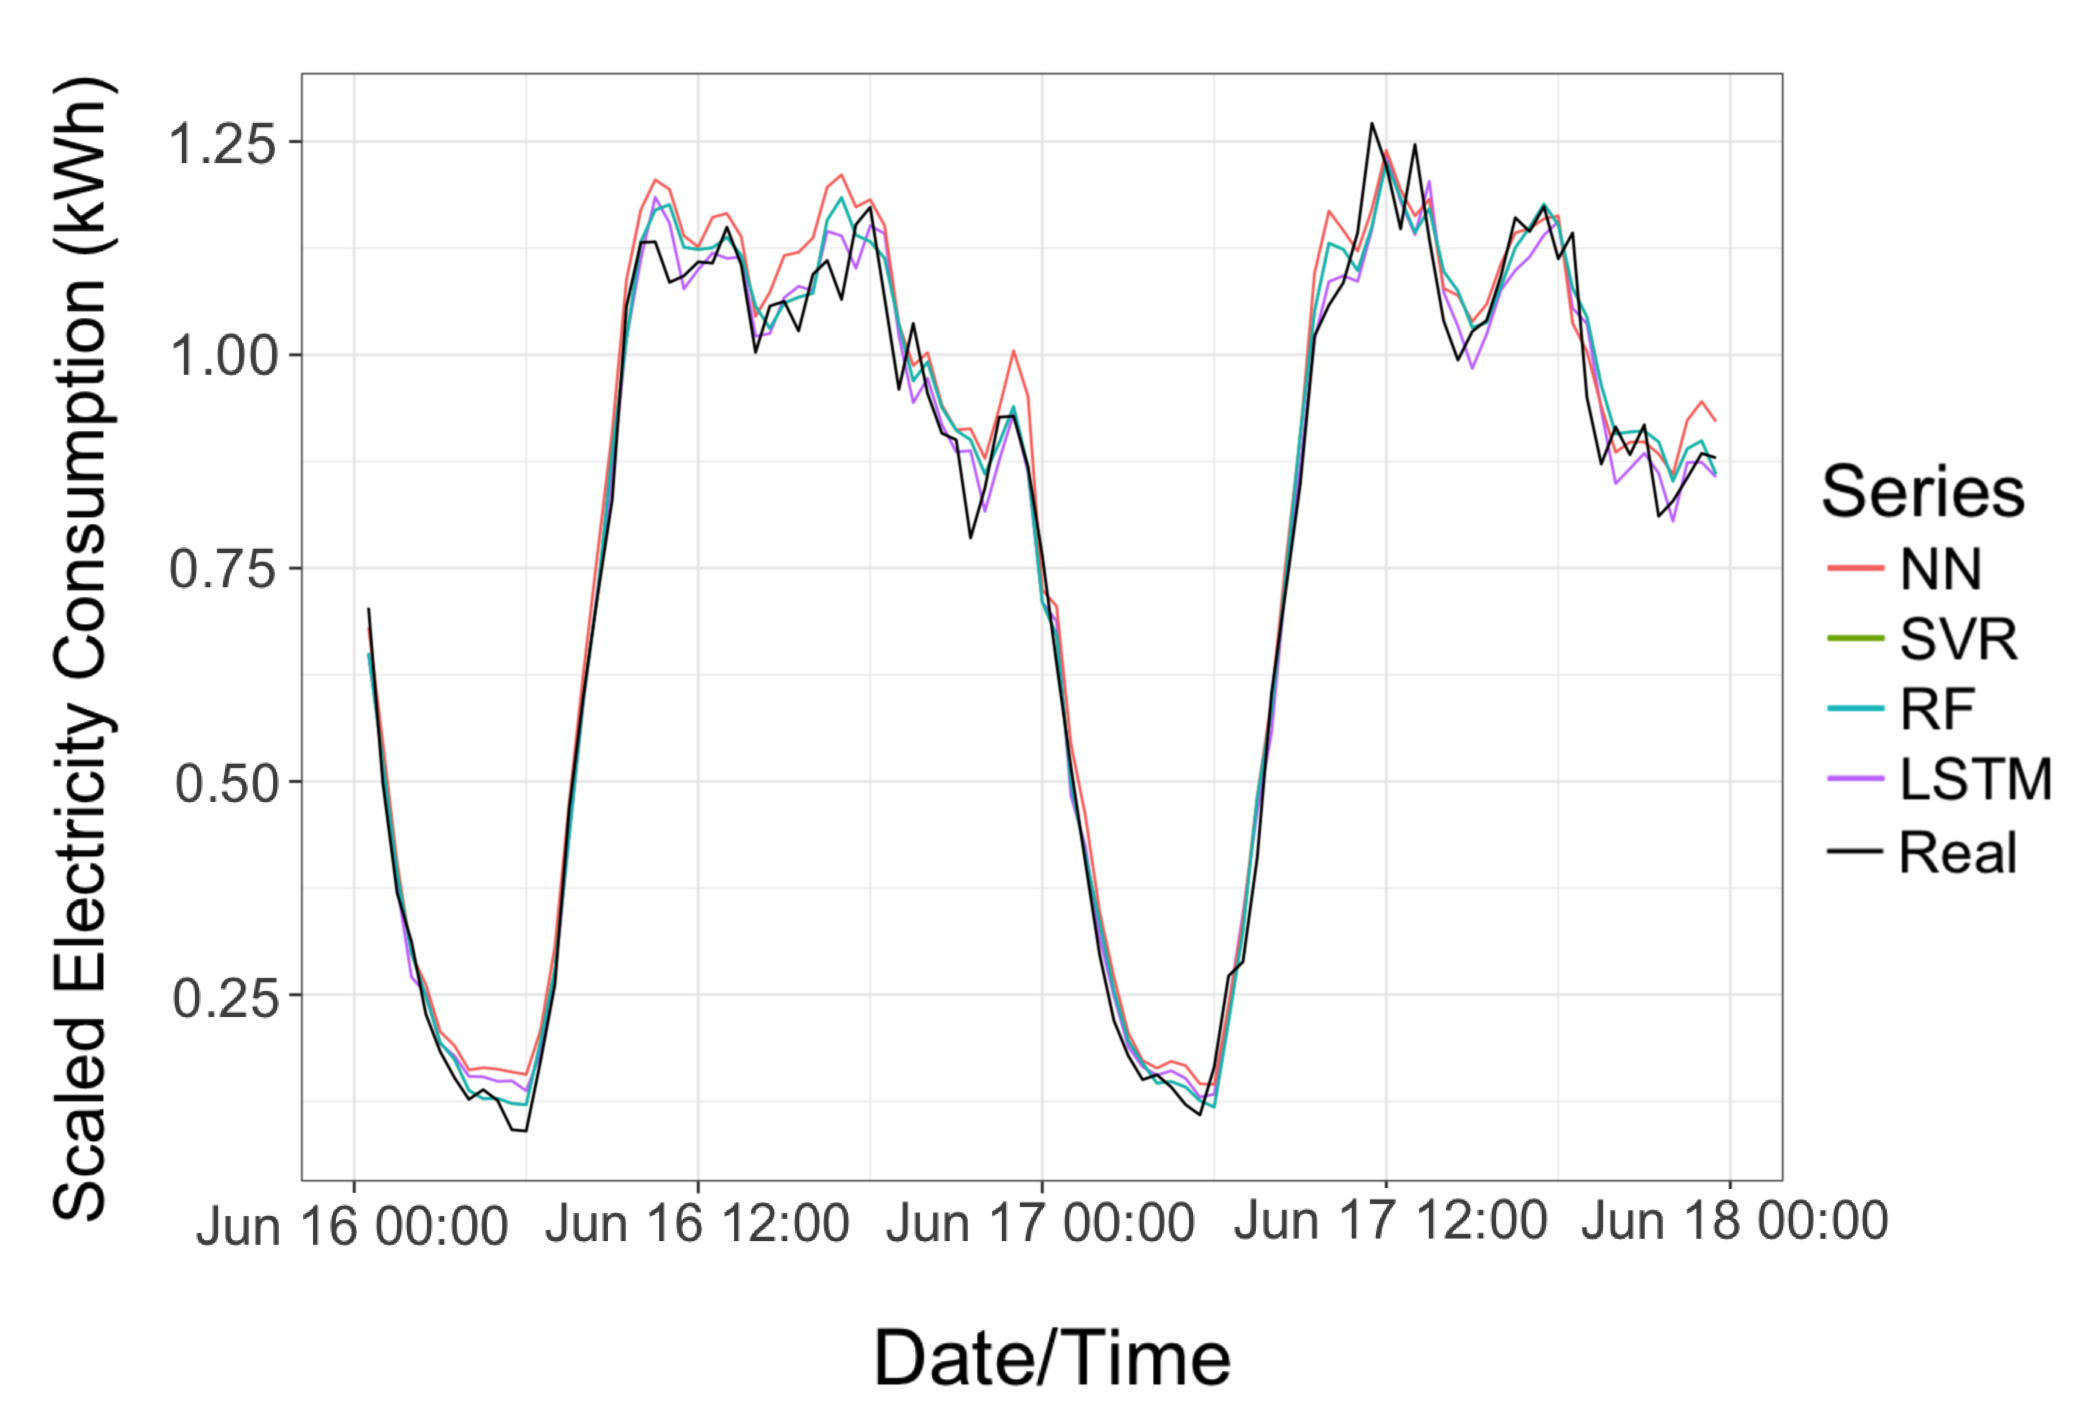
\includegraphics[width=0.8\textwidth]{Chapter5/figures/actual_vs_predicted_enlarged.png}
	\caption{Real electricity consumption versus predicted electricity consumption between June 16th and June 18th 2010.}
	\label{fig:act_vs_pred}
\end{figure}

The impact of using calendar attributes improves prediction accuracy by 6\% for neural networks, 4\% for Random Forests and 1\% for SVR. For these results please see figure \ref{appendix:calendar_attr} in appendix \ref{appendix:results}.

It is proposed that the optimum value for \textit{k} cluster centres was four due to the distinct patterns observed in each of the clusters. At $k=5$ one of the distinct clusters is split, and leads to an increase in stochasticity. At $k=3$ the stochasticity is also increased by the aggregation of load profiles which are dissimilar. % To see a breakdown of the average clusters please refer to figure \ref{appendix:clustercentre} in appendix \ref{appendix:results}.

However, the optimum number of clusters will vary for different datasets. Differing geographies may display varying usage characteristics due to culture, weather or social norms.

The results demonstrate that SVR, Random Forests and the ANN have similar accuracy, and adequately predict electricity consumption. The LSTM shows a similar pattern in increasing accuracy with number of clusters, but performs worse than the other models. The Random Forest seems to outperform each of the other models. This may be due to the internal operation of the Random Forest which undertakes its own cross-validation using out-of-bag samples. 

Figure \ref{fig:act_vs_pred} displays actual electricity consumption versus predicted results. It shows that the LSTM model predicts a similar value in the next time step as the previous time step, which would explain its inferior results to the other models.  

The training times were tested by timing how long the models took to fit for four clusters. The Support Vector Regression took less time than all of the other methods, whereas the LSTM took the longest. The Support Vector Regression model required 3 minutes and 18 seconds to run. The Random Forest required 14 minutes and 58 seconds. The Artificial Neural Network required 17 minutes and 48 seconds, whilst the LSTM took 21 minutes 11 seconds to run.

The time to make a single prediction was recorded at sub microseconds and therefore deemed negligible for our use-case.

\section{Conclusion}

The availability of data produced by smart meters enables network operators to gain greater insights into their customer behaviour and electricity usage. We demonstrated that implementing the \textit{k}-means clustering algorithm to group similar customers improved the accuracy of the models tested. Distinct models were trained for each cluster and the individual forecasts aggregated for the total aggregated forecast. It was found that Random Forests outperformed all other models at each level of clustering. The optimum number of clusters was found to be four. Whilst the dataset used focused on residential data it is expected that applying a similar clustering technique on commercial properties would have a similar effect.

It is considered that monthly retraining of the models would be required to ensure continued accuracy. However, this is not expected to be a problem due to the short time time required for model training. Once trained, the prediction times are negligible.

In future work, we will look into the features that best aid in the forecasting of electricity consumption, try a wider variety of models in an ensemble manner and try different clustering techniques such as self-organizing maps (SOM) to obtain better accuracy results. We will also compare a greater variety of forecasting metrics.

% To utilize more of the data and increase the number of models trained these results could be run in parallel in future.




